\documentclass[9pt,tutorial]{Styling/livecoms}
%\documentclass[10pt,twocolumn]{article}
\usepackage{chngcntr}
\counterwithout{figure}{section}
\DeclareCaptionLabelFormat{custom}{Figure #2}
\captionsetup[figure]{labelformat=custom}
\usepackage{caption}
\usepackage{courier}
\usepackage{enumitem}
\usepackage{hyperref}
\usepackage{listings}
\lstset{showstringspaces=false}
\usepackage[italic]{mathastext}
\usepackage[version=4]{mhchem}
\usepackage{multicol}
\usepackage{natbib}
%\usepackage{siunitx}
\usepackage[skins]{tcolorbox}
\usepackage[normalem]{ulem}
%\usepackage{upgreek}
\usepackage{wrapfig}
\usepackage{xcolor}

\newlist{todolist}{itemize}{2}
\setlist[todolist]{label=$\square$}

% Special commands and macros
\graphicspath{{Figures/}}
%\DeclareSIUnit\Molar{M}

\setlistdepth{9}
\newlist{myEnumerate}{enumerate}{9}
\setlist[myEnumerate,1]{label=\arabic*}
\setlist[myEnumerate,2]{label=\arabi*}
\setlist[myEnumerate,3]{label=(\Alph*)}
\setlist[myEnumerate,4]{label=(\roman*)}
\setlist[myEnumerate,5]{label=(\alph*)}
\setlist[myEnumerate,6]{label=(\arabic*)}
\setlist[myEnumerate,7]{label=(\Roman*)}
\setlist[myEnumerate,8]{label=(\Alph*)}
\setlist[myEnumerate,9]{label=(\roman*)}

\hypersetup{
    colorlinks=true,
    linkcolor=blue,
    filecolor=magenta,
    urlcolor=cyan,
    pdftitle={SAFEP Tutorial},
    hypertexnames=false,
    }

\newcommand{\sourcefile}{\path}

%Commenting commands
% \newcommand{\jh}[1]{\textcolor{blue}{JH: #1}}
% \newcommand{\grace}[1]{\textcolor{red}{GB: #1}}
% \newcommand{\Mina}[1]{\textcolor{magenta}{Mina: #1}}
% \newcommand{\jesse}[1]{\textcolor{green}{Jesse: #1}}
%\newcommand{\ezry}[1]{\textcolor{orange}{Ezry: #1}}

%Formatting macros
\newcommand{\terminal}[1]{\texttt{\$#1}}
\newcommand{\tkconsole}[1]{\texttt{\%#1}} 
\newcommand{\filepath}[1]{\textit{#1}}

\newtcbox{\inlineBox}[1][]{colback=#1!10!white, colframe=#1!50!black, enhanced,nobeforeafter,tcbox raise base,boxrule=0.4pt,top=0mm,bottom=0mm,right=0mm,left=0mm,arc=1pt,boxsep=2pt, sharp corners}
\MakeRobust\inlineBox

\newcommand{\button}[1]{
  \inlineBox[gray]{\texttt{#1}}
}
\definecolor{dark-gray}{gray}{0.2}
\newcommand{\menu}[1]{
  \textit{#1}
}
\newcommand{\option}[1]{
  \texttt{#1}
}
\newcommand{\textInput}[1]{
  \texttt{#1}
}

\newcommand{\exponential}[1]{\exp\left[#1\right]}


\newcommand{\githubrepository}{\url{https://github.com/jhenin/SAFEP_tutorial}}


\title{Computing Absolute Binding Affinities by Streamlined Alchemical Free Energy Perturbation}

\author[1\authfn{1}]{Ezry Santiago-McRae}
\author[2,3,4\authfn{1}]{Mina Ebrahimi}
\author[1]{Jesse W. Sandberg}
\author[1,5\authfn{2}]{Grace Brannigan}
\author[3,4\authfn{2}]{Jérôme Hénin}
\affil[1]{Center for Computational and Integrative Biology, Rutgers University, Camden, New Jersey, 08102}
\affil[2]{Department of Physical Chemistry, School of Chemistry, College of Science, University of Tehran, Tehran 1417935840, Iran}
\affil[3]{Université Paris Cité, Laboratoire de Biochimie Théorique, CNRS UPR 9080, 75005, Paris, France}
\affil[4]{Institut de Biologie Physico-Chimique -- Fondation Edmond de Rothschild, PSL Research University, Paris, France}
\affil[5]{Department of Physics, Rutgers University, Camden, New Jersey, 08102}

\corr{grace.brannigan@rutgers.edu}{GB}
\corr{jerome.henin@cnrs.fr}{JH}

\orcid{Ezry Santiago-McRae}{0000-0002-0930-8277}
\orcid{Mina Ebrahimi}{0000-0001-6204-5886}
\orcid{Jesse W. Sandberg}{0000-0001-7466-8466}
\orcid{Grace Brannigan}{0000-0001-8949-2694}
\orcid{J\'er\^ome H\'enin}{0000-0003-2540-4098}

\contrib[\authfn{1}]{These authors contributed equally to this work}
\contrib[\authfn{2}]{These authors played an equal role in supervising this work}

\blurb{This LiveCoMS document is maintained online on GitHub at \githubrepository; to provide feedback, suggestions, or help improve it, please visit the GitHub repository and participate via the issue tracker.}

%%%%%%%%%%%%%%%%%%%%%%%%%%%%%%%%%%%%%%%%%%%%%%%%%%%%%%%%%%%%
%%% PUBLICATION INFORMATION
%%% Fill out these parameters when available
%%% These are used when the "pubversion'' option is invoked
%%%%%%%%%%%%%%%%%%%%%%%%%%%%%%%%%%%%%%%%%%%%%%%%%%%%%%%%%%%%
% \pubDOI{10.XXXX/YYYYYYY}
% \pubvolume{<volume>}
% \pubissue{<issue>}
% \pubyear{<year>}
% \articlenum{<number>}
% \datereceived{Day Month Year}
% \dateaccepted{Day Month Year}

\begin{document}

\begin{frontmatter}
\maketitle
\begin{abstract}
    Free Energy Perturbation (FEP) is a powerful but challenging computational technique for estimating differences in free energy between two or more states.
    This document is intended both as a tutorial and as an adaptable protocol for computing free energies of binding using free energy perturbations in NAMD.
    We present the Streamlined Alchemical Free Energy Perturbation (SAFEP) framework. SAFEP shifts the computational frame of reference from the ligand to the binding site itself. 
    This both simplifies the thermodynamic cycle and makes the approach more broadly applicable to superficial sites and other less common geometries.
    As a practical example, we give instructions for calculating the absolute binding free energy of phenol to lysozyme. 
    We assume familiarity with standard procedures for setting up, running, and analyzing molecular dynamics simulations using NAMD and VMD.
    While simulation times will vary, the human tasks should take no more than 3 to 4 hours for a reader without previous training in free energy calculations or experience with the Colvars Dashboard.
    Sample data are provided for all key calculations both for comparison and readers' convenience.
\end{abstract}
\end{frontmatter}

\section{Introduction}
In this tutorial we are principally concerned with computing the Absolute Binding Free Energy (ABFE) of a ligand to its receptor. 
While many methods of measuring free energies exist, alchemical Free Energy Perturbation (FEP) methods make use of the fact that, since the change in free energy is path independent, it can be calculated via an unphysical path. In the case of FEP, that unphysical path is defined by scaling the non-bonded interactions of the ligand.\cite{Gilson1997, Mey2020, Hamelberg2004, Woo2005, Hermans1986, Deng2006}
In essence, the user can make a bound ligand ``disappear'' from the binding site, make it re-appear in the bulk solution, and calculate the corresponding free energy difference. 

While elegant and exact in principle, FEP calculations are often unwieldy in practice.
One of the most stubborn challenges that most FEP implementations face is that the ligand must maintain the original bound configuration during decoupling, even as the very interactions that stabilize the bound configuration are weakened.
Consequently, absolute binding schemes introduce restraints on the ligand to mimic the interactions that stabilize the bound ensemble. 
While there are many such schemes to accelerate convergence,\cite{Henin2017,Hermans1997,Boresch2003, Fu2017} most do so in ways that require error-prone manual parameterization and many hours of the user's time.
Many of these techniques have already been reviewed by Mey et al. \cite{Mey2020} 
As discussed there, no restraint scheme is without cost; the restraints themselves will bias the estimated free energy and must be corrected in the coupled state, the decoupled (gas phase) state, or both.
Broadly, simple, mutually orthogonal restraints (e.g. \cite{Boresch2003, Salari2018}) can be corrected analytically, while more collective restraints (e.g. the DBC) must be corrected numerically.\cite{Salari2018, Fu2017}
%Boresch restraints, for example, can be introduced during decoupling and corrected for analytically,\cite{Boresch2003} while more collective restraint schemes like layered restraints \cite{Fu2017} or our own Distance-to-Bound Configuration restraint \cite{Salari2018} must be corrected numerically as discussed below. 

Streamlined Alchemical Free Energy Perturbation (SAFEP) is specifically designed to make FEP calculations faster and easier for the user without sacrificing accuracy of the final free energy estimate.
SAFEP reduces conceptual and computational complexity by replacing conventional rotational and translational restraints for stabilizing the ligand in the binding site with a single Distance-to-Bound Configuration (DBC) coordinate.
This makes setup easier because, instead of parameterizing six or more individual restraints, the user need only parameterize one.
Furthermore, SAFEP can handle superficial binding sites in phase-separated bulk with atomistic resolution. \cite{Salari2018}
Statistically optimal FEP estimators require both decoupling and recoupling calculations; SAFEP uses Interleaved Double-Wide Sampling (IDWS) to extract both quantities from the same calculation, roughly halving the required simulation time. \cite{Bernardi2020} (see the \href{https://www.ks.uiuc.edu/Research/namd/2.14/ug/node64.html}{NAMD User Guide Free Energy Perturbation})
SAFEP makes extensive use of the Colvars Dashboard in VMD, allowing the user to easily measure collective variables, impose biases, and generate restraint configuration files from one interface~\cite{Henin2022}. 
Finally, analysis tools and data visualizations are included in one Jupyter notebook allowing for comprehensive quality assurance along with the $\Delta G$ calculation.

Figure \ref{fig:cycle} depicts the thermodynamic paths at the heart of SAFEP. 
The desired quantity $\Delta G^\circ_\mathrm{bind}$ (red, left column) is equal to the sum of the steps in the SAFEP method (black, right column), as shown in equation \ref{eq:overalldG}. 
\begin{equation}\label{eq:overalldG}
    \color{red} \Delta G^\circ_\mathrm{bind} = \color{black} - \Delta G_\mathrm{site}^* + \Delta G_\mathrm{DBC} - \Delta G^\circ_\mathrm{V} + \Delta G^*_\mathrm{bulk} 
\end{equation}
\noindent This equation forms the basis for the steps that follow in this tutorial. 

\begin{figure}[!ht]
    \centering
    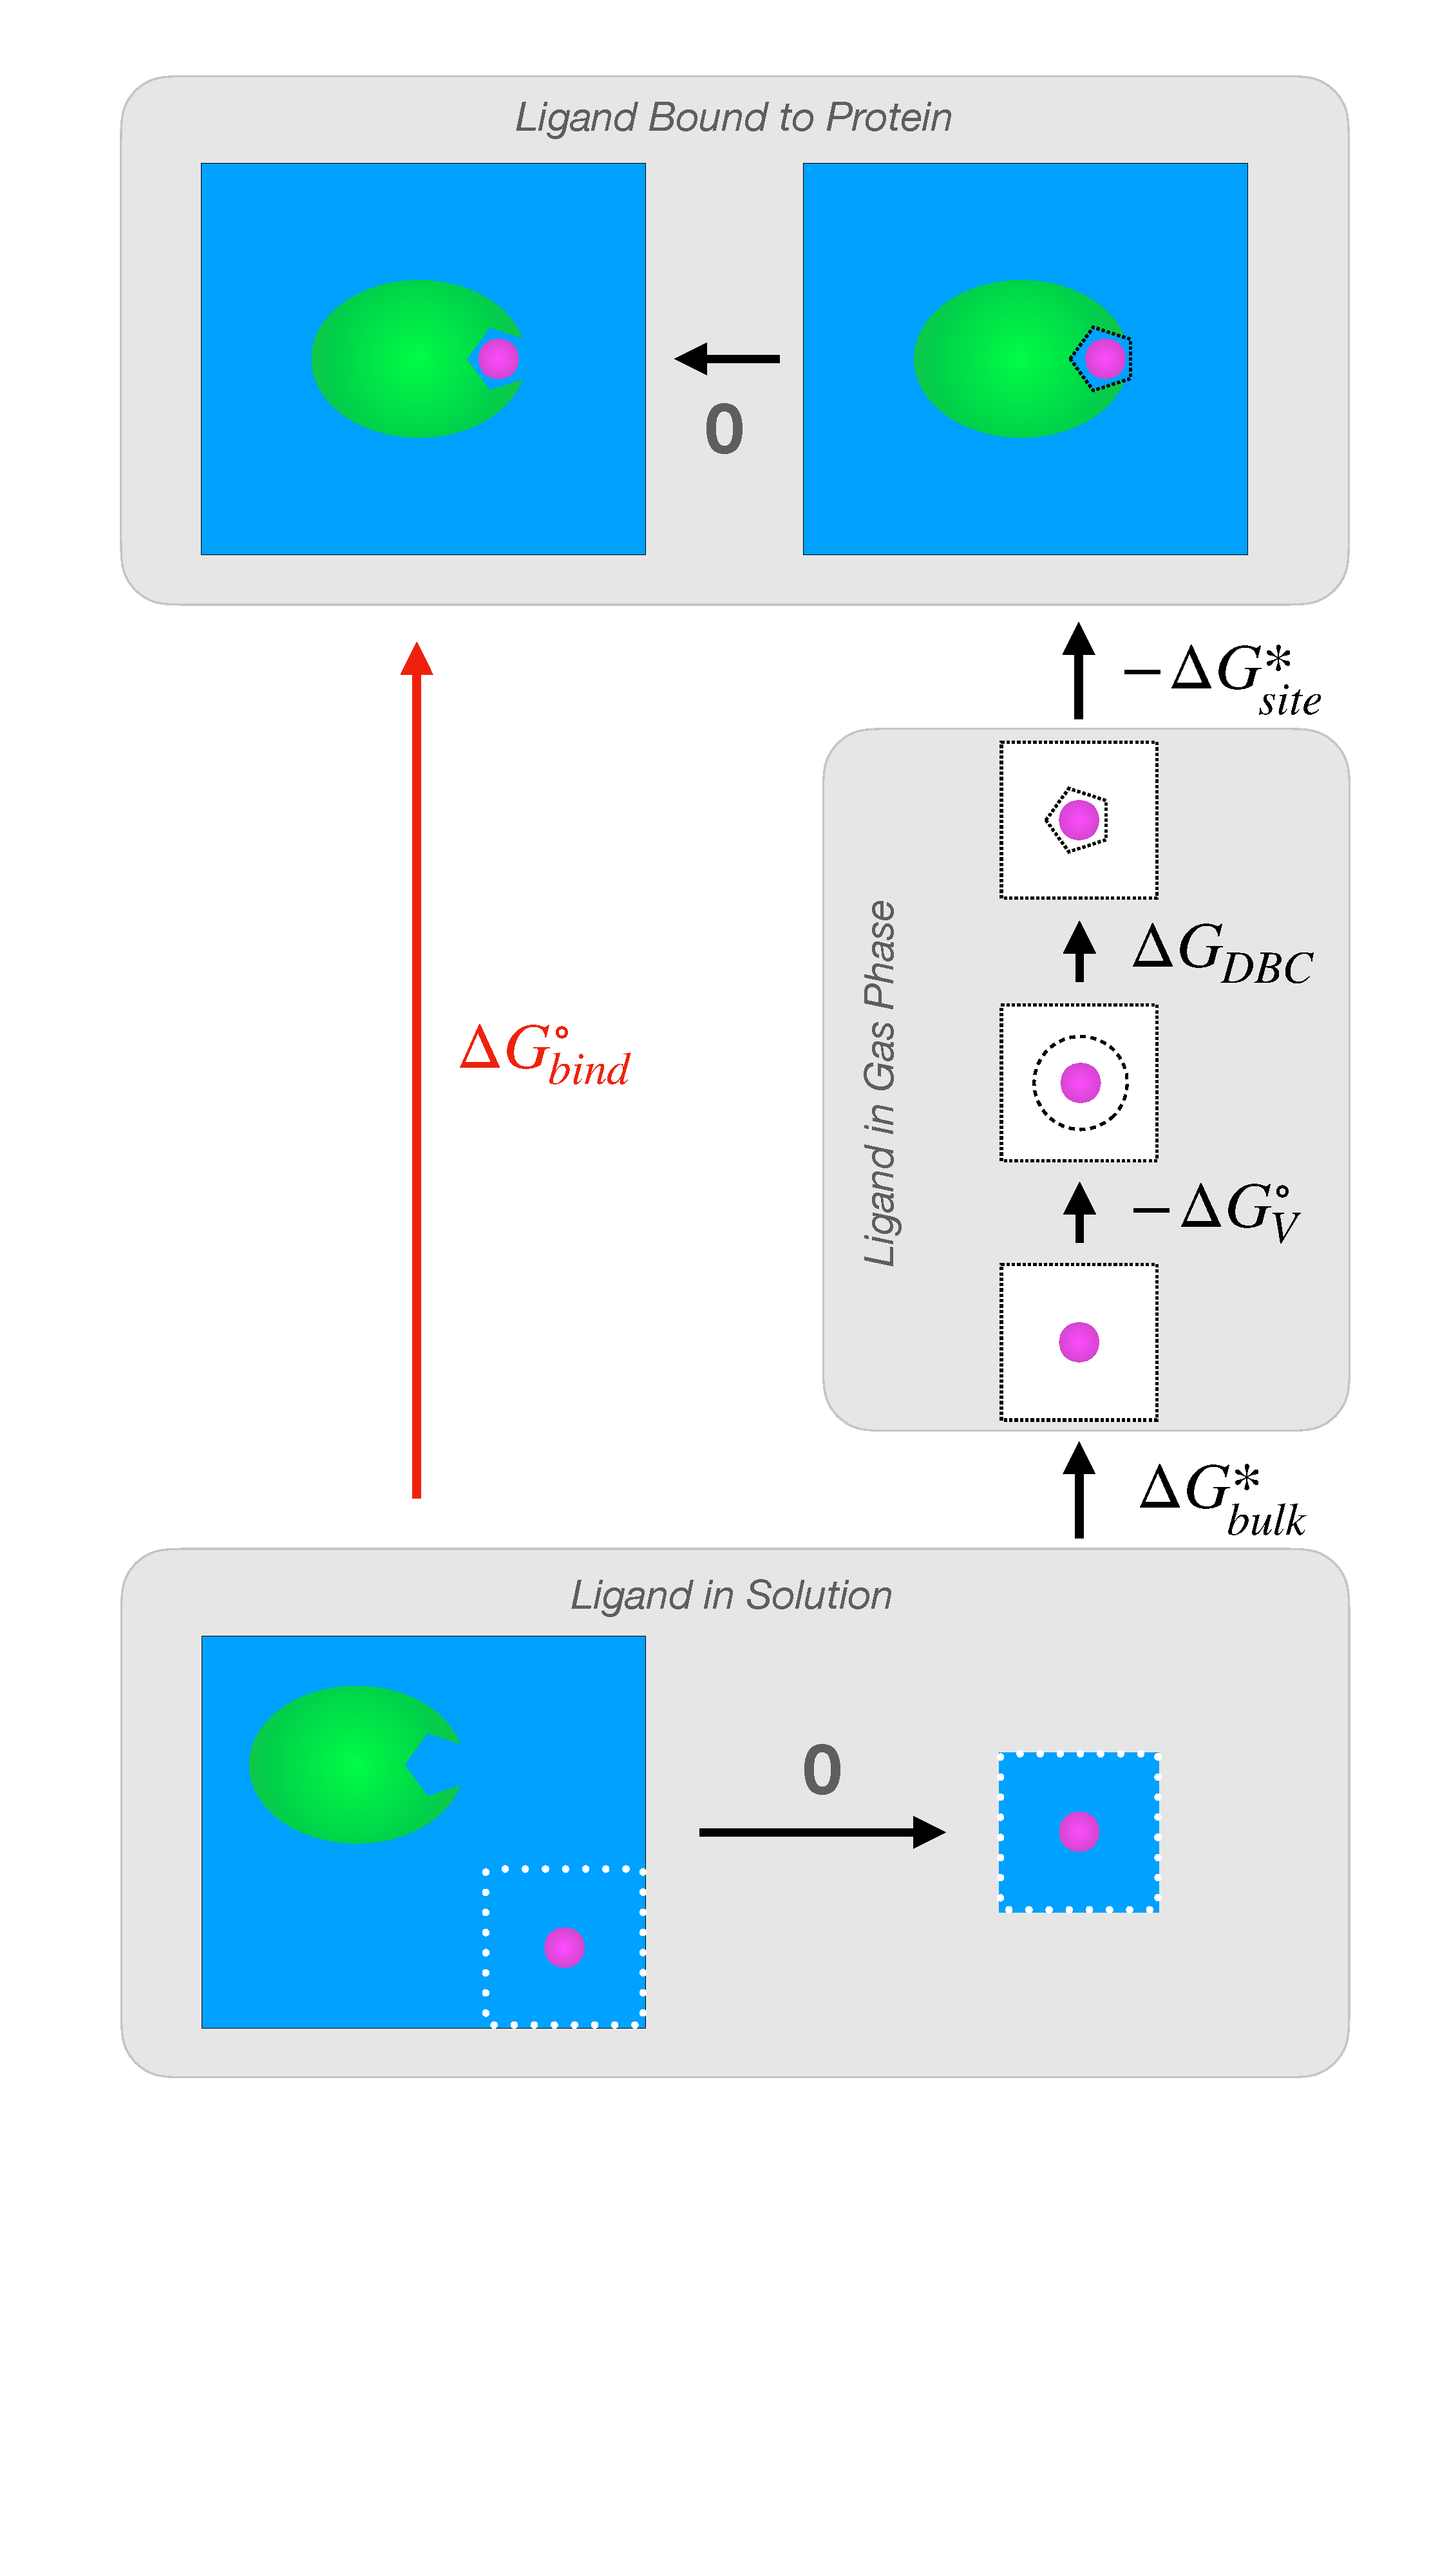
\includegraphics[width=0.5\textwidth]{SAFEP_cycle.pdf}
    \caption{\textbf{The SAFEP thermodynamic cycle.} 
    Computing the ABFE of a ligand bound to a protein ($\Delta G^\circ_\mathrm{bind}$) is the ultimate goal. 
    This is found by computing the free energies of several, smaller perturbations: 1) decoupling the unbound ligand from the condensed phase to the gas phase under no restraints ($\Delta G^*_{\mathrm{bulk}}$); 2) enforcing a restraint scheme ($-\Delta G^\circ_\mathrm{V}$ and $\Delta G_\mathrm{DBC}$); and 3) coupling the ligand from the gas phase to its bound pose in the condensed phase (-$\Delta G^*_{\mathrm{site}}$) under the Distance-to-Bound Configuration (DBC) restraint.
    The free energy contribution of the volumetric restraint ($\Delta G^\circ_\mathrm{V}$) is calculated analytically, while the other three contributions are calculated via simulation.The free energy of the top horizontal leg vanishes in SAFEP due to design of the DBC restraint. See \ref{app:restraints} for more details.}
    \label{fig:cycle}
\end{figure}

\subsection{Scope}
The following steps will walk the user through the calculation of an Absolute Binding Free Energy (ABFE) using a computationally affordable example (phenol bound to a mutant lysozyme), but we have written these steps to be straightforward to generalize to other systems.
These exact steps have been tested thoroughly for this particular system.
More detailed descriptions of for each step can be found in \hyperref[app:motivation]{Appendices A-E}. Similarly, to facilitate generalization of the method to other systems, we have provided a checklist in \ref{app:checklist} and additional troubleshooting advice in \ref{app:troubleshooting}, as well as template files for the user to adapt in the common directory of the GitHub.

More detailed descriptions and justifications for each step are provided in further appendices. These appendix entries are also hyperlinked and referenced throughout the body of the tutorial.

\subsection{Prerequisites}
    \subsubsection{Background knowledge}\label{sec:prerequisites}
    
    We assume intermediate experience with running classical MD with NAMD 2.14 or later. If this is not the case, please see the NAMD Tutorial \cite{phillips2003}. The latter portions that involve analysis are less important for this tutorial. Useful, but not required, material on alchemical free energy perturbations can be found in “\textit{In-silico} alchemy: A tutorial for alchemical free-energy perturbation calculations with NAMD” \cite{Henin2017}. Finally, basic knowledge of VMD and Python will be required for data analysis and visualization.  

\subsubsection{Software requirements}\label{sec:7.2}
    \begin{enumerate}
        \item NAMD 2.14 or later. Support for GPU-accelerated (CUDA) alchemy with IDWS is available in NAMD 3 but is not yet fully validated.
        \item \textbf{VMD 1.9.4.a57} or later. Slightly older versions of VMD may be used, but will require manual update of the Colvars Dashboard. See the Colvars Dashboard \href{https://github.com/Colvars/colvars/tree/master/vmd/cv_dashboard}{README} for more information on getting the latest version. 
        \item Python 3.9.12 or later
        \item Jupyter
        \item safep Python package and its dependencies:
        \begin{enumerate}
        \item Alchemlyb
        \item Glob
        \item MatPlotLib
        \item Numpy 1.22 or later
        \item Pandas
        \item PyMBAR
        \end{enumerate}
    \end{enumerate}

NAMD will be used to perform simulations. GPU acceleration of restrained free energy perturbations are expected in NAMD3 alpha 14 (with \textInput{CUDASOAintegrate off}) \cite{Chen2020, Phillips2020}. System setup, trajectory visualization, and restraint definition will be carried out in VMD \cite{Humphrey1996}. Data analysis and visualization will be handled by a Jupyter notebook with the above dependencies.

High-performance computing resources are recommended, but not required. Sample outputs are provided for each step for users with limited compute resources or time.

\subsection{Process Overview} \label{sec:processOverview}

Within the scope of free energy perturbations, absolute free energies of binding are typically calculated by the double-decoupling method (DDM) \cite{Gilson1997, Hamelberg2004, Woo2005}. 
In this method, pair interactions (non-bonded terms) between the ligand and the rest of the simulation box are gradually scaled to zero (decoupled) from both a bound state and an unbound, solvated state.

In order to maintain the ligand in its bound state, most current approaches introduce a series of rotational and translational restraints on the ligand, each of which requires parameterization and an additional $\Delta G$ correction.
In contrast, SAFEP uses just one restraint: a flat well on the ``Distance-to-Bound Configuration'' (DBC). This minimizes both the number of parameters to be optimized and reduces the number of simulations to be performed compared to layered restraints (See Figure \ref{fig:DBC} or \ref{app:restraints} for details).

The thermodynamic cycle used for absolute binding free energies in SAFEP is seen in Figure \ref{fig:cycle} while the unknown values (black arrows) can be calculated by the simulations outlined in Figure \ref{fig:workflow}.
More precisely, the thermodynamic cycle (Fig \ref{fig:cycle}) and the corresponding simulations (Fig \ref{fig:workflow}) are broken into three main steps involving three simulation systems: 1) the ligand bound to the protein, 2) the ligand in the gas phase, and 3) the ligand in the bulk. 
The order of computations is unimportant so long as the end-points are defined consistently (e.g. the same temperature is used throughout and restraints are used consistently). 
For the sake of clarity, we have arranged the process linearly: Steps A and B are concerned with calculating $\Delta G^*_\mathrm{site}$; step C addresses the free energy of the DBC ($\Delta G_\mathrm{DBC}$); step D measures $\Delta G^*_\mathrm{bulk}$; and step E calculates an analytical correction ($\Delta G^\circ_\mathrm{V}$) and combines all the preceding terms into the overall $\Delta G^\circ_\mathrm{bind}$ using Equation~\ref{eq:overalldG}.


% \begin{table}[H]
%     \centering
%     \caption{Acronym Definitions}
%     \label{tab:variables}
%     \begin{tabular}{  p{.2\linewidth} | p{.7\linewidth}  }
%         Variable & Definition\\
%         \hline
%         SAFEP & Streamlined Alchemical Free Energy Perturbations\\
%         \hline
%         DBC & Distance-to-Bound-Configuration \\
%         \hline
%         COM & Center Of Mass (displacement)\\
%         \hline
%         [A]FEP & [Alchemical] Free Energy Perturbation \\
%         \hline
%         TI & Thermodynamic Integration\\
%     \end{tabular}
% \end{table}

\onecolumn
\begin{figure}[h]
    \centering
    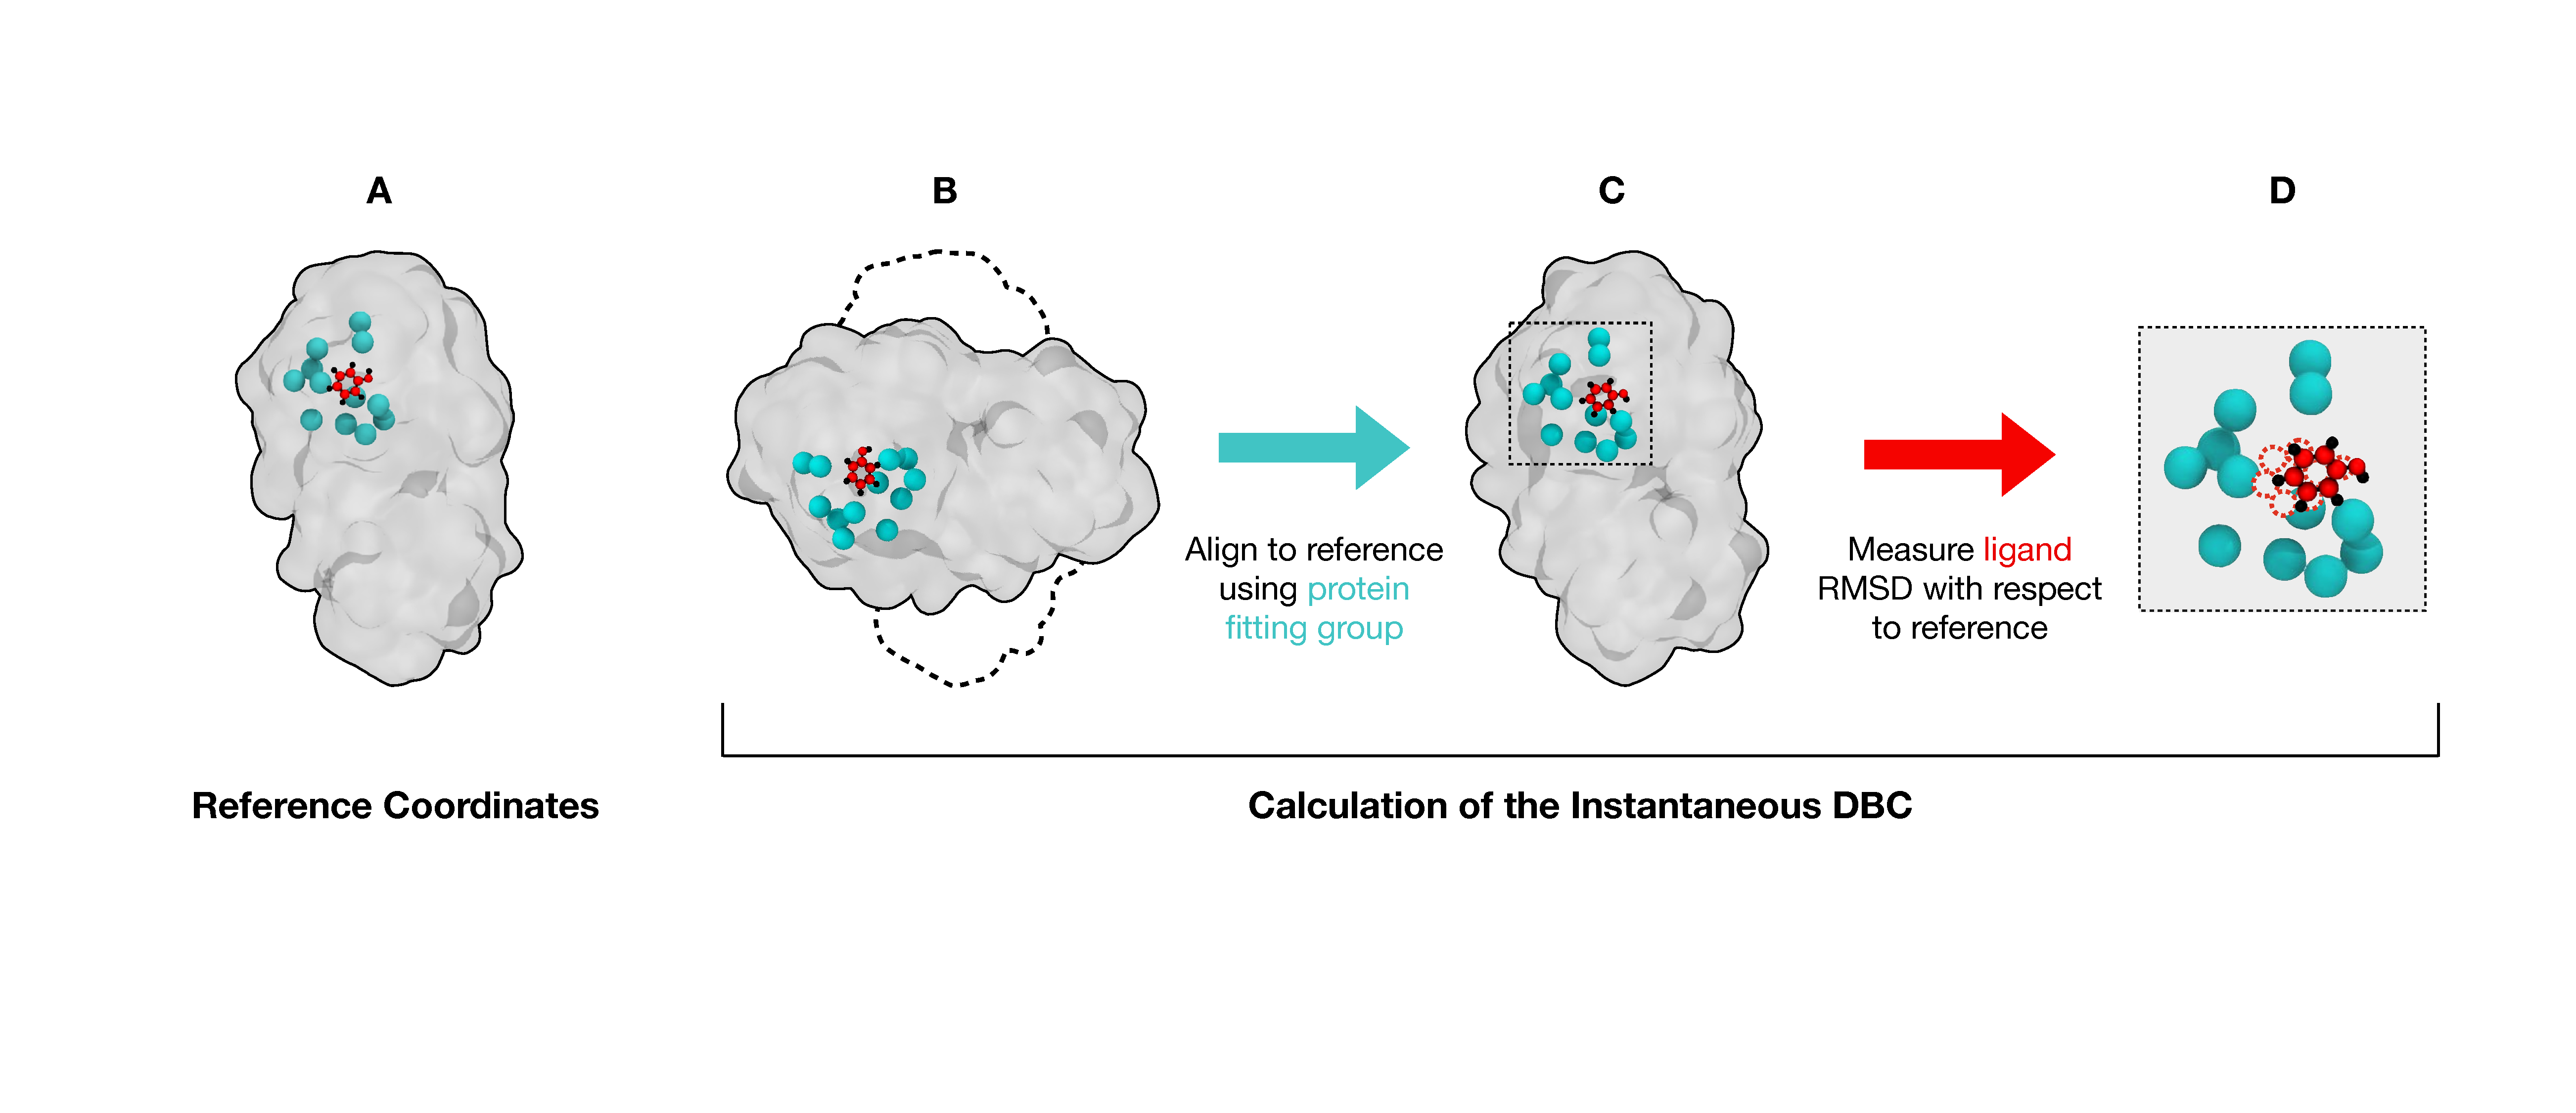
\includegraphics[width=\textwidth]{DBCfigfinal.pdf}
    \caption{\textbf{The Distance-to-Bound-Configuration (DBC) coordinate.} The DBC coordinate is used as a bias to prevent ligand dissociation during uncoupling. The user specifies a subset of protein atoms as the fitting group (teal) and a subset of ligand atoms (red); also shown are the protein surface (gray) and remaining ligand atoms (black). A) User-specified reference coordinates for both protein and ligand.    %and User-specified fitting group atoms (teal), restrained ligand atoms (red), and other ligand atoms (black) reference coordinates. 
    B) During simulation, both protein and ligand will drift from the reference coordinates (black dashed outline).   
    C) In order to remove rotational and translational diffusion of the protein from calculation of the DBC, Colvars aligns the system to the reference coordinates using only the protein fitting group atoms. 
    D) The DBC is the RMSD of the user-specified ligand atoms (solid) with respect to the reference coordinates (dashed).}
    \label{fig:DBC}
\end{figure}
\twocolumn
\begin{figure}[h]
    \centering
    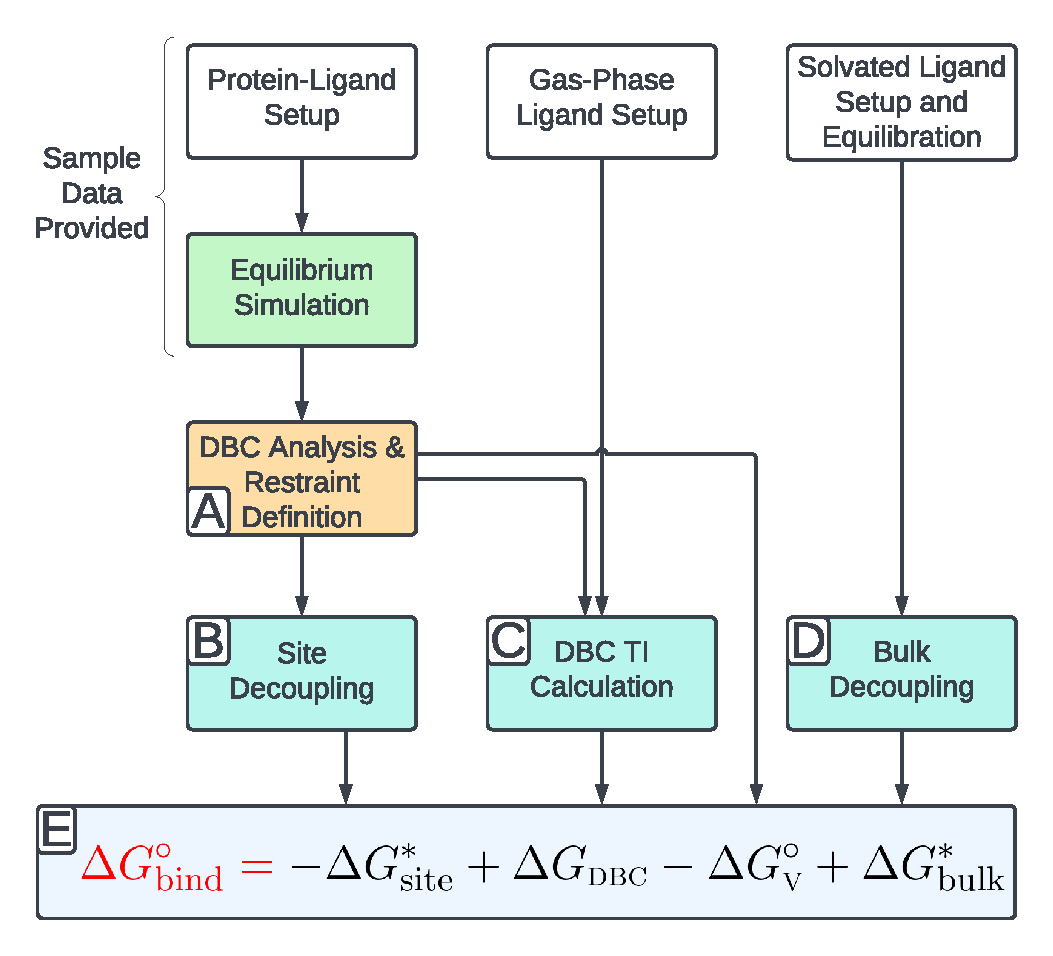
\includegraphics[width=.9\linewidth]{CoarseGrainedWorkflow.pdf}
    \caption[test]{\textbf{The overall SAFEP workflow.} The dependencies in this flowchart can be used to decide in what order steps can be performed, and which simulations can be run simultaneously. From top to bottom and left to right: 1) the ligand must be setup (as for classical MD) in each of the three states (bound, solvated, gas phase) and minimally relaxed (white boxes); 2) a longer, unbiased simulation of the ligand-protein complex is necessary to sample the bound state (green box) which is used to determine the distribution of the DBC (orange box, \ref{step:equilibrium}); 3) two FEP calculations and a thermodynamic integration (TI) calculation are carried out (blue boxes, \ref{step:proteinDecouple}, \ref{step:restraintPerturbation}, and \ref{step:bulkDecoupling}); and 4) the resulting values are combined to get the standard free energy of binding (gray box; \ref{step:combinequantities}).}
    \label{fig:workflow}
\end{figure}
\onecolumn
\section{Protocol} \label{sec:protocol}
%\hline
\vspace{0.5em}

%\hline\\
The following steps demonstrate the SAFEP protocol applied to a computationally affordable example: calculating the binding affinity of phenol to a lysozyme mutant.
For more details on the rationale behind this choice, see \ref{app:motivation}.

\textbf{Procedure:}
\begin{enumerate}
    \item \textbf{Clone the \href{https://github.com/jhenin/SAFEP_tutorial}{SAFEP\_tutorial repository} to your local environment} Tip: use \textInput{-{}-depth 1} to avoid downloading the entire commit history. \\
    \textInput{git clone https://github.com/jhenin/SAFEP\_tutorial.git -{}-depth 1}
    \item \textbf{Navigate to the cloned repo}\\
    This is the starting path for all command line prompts in this tutorial. \\
    \textInput{cd SAFEP\_tutorial}
    \item \textbf{Install the SAFEP package by running:}\\
    \textInput{pip install git+https://github.com/BranniganLab/safep.git}
    \item \textbf{Tips:} 
    \begin{itemize}
    \item All run.namd files contain a line that reads \textInput{set useSampleFiles 0}. To use the sample data provided, set the value to 1. Otherwise, NAMD will use your inputs (provided they are named exactly as described in this document).
    \item If you run VMD and your simulations on different computers, then you will need to manually edit paths later when you are running simulations. 
    \item Some simulations will take several days on a single core. To use 4 cores in parallel we have included the \textInput{+p4} argument in the commands for the longer NAMD runs. This number may need to optimized for your particular compute resources.
    \item Common settings used by multiple simulations are in \filepath{common/common\_config.namd}, which is sourced by the individual configuration files. This simplifies the individual configuration files and ensures consistency between calculations, which is a critical part of any free energy method.
    \item [Old versions of Colvars Dashboard only] Colvars has a functionality called ``auto-update selections.'' Please turn it off by deleting the comment line that begins ``auto-updating'' in all Colvar config files. It is by default in newer CV Dashboard versions.
    \end{itemize}
    \item \textbf{Move on to \hyperref[step:equilibrium]{Step A}}
\end{enumerate}

\renewcommand\thesubsection{Step \Alph{subsection}}
\subsection{\hspace{-1em}: Sample the bound state and define the binding restraint}\label{step:equilibrium}
    \begin{tcolorbox}[colback=blue!5!white,colframe=blue!75!black] 
    Alchemical decoupling removes the interactions that stabilize the occupied ensemble. 
    Consequently, during decoupling the ligand may spontaneously diffuse into the bulk. 
    Therefore, we need to impose an external restraint to force the ligand to occupy the bound state throughout decoupling. 
    With SAFEP we apply a single restraint on the Distance-to-Bound Configuration (DBC) collective variable as illustrated in Fig. \ref{fig:DBC}. 
    This restraint which is straightforward to define and relatively insensitive to small differences in parameters \cite{Salari2018}.
    Its sole correction factor is calculated via Thermodynamic Integration later in this tutorial. 
    For more details about the DBC restraint see \ref{app:restraints} and \cite{Salari2018}. 
    For a discussion of the merits in accounting for symmetry when computing the DBC of a small, symmetric ligand see \ref{app:Symmetry} and \cite{Ebrahimi2022}.
    \end{tcolorbox}
    
    \noindent{\textbf{Required Input:}}  
    \begin{itemize}
        \item Structure file: \filepath{common/structures/phenol\_lysozyme.psf} \item Coordinate file: \filepath{common/structures/phenol\_lysozyme.pdb}
        \item Equilibrium trajectory: \filepath{stepA\_create\_DBC/inputs/unbiased-sample.dcd}
    \end{itemize}
    \textbf{Essential Output:}
    \begin{itemize}
        \item DBC restraint parameters: \filepath{stepA\_alchemy\_site/outputs/DBC\_restraint.colvars}
    \end{itemize}
    \textbf{Procedure:}
    \begin{enumerate}
    \setcounter{enumi}{-1}
    \item \textbf{Run standard MD of the occupied state.}\label{step:unbiased}\\
    This simulation should be long enough ($\sim$50 ns) for the ligand to explore the configuration space of the bound state. See \ref{app:equilibration} for more details.
    \textbf{Note: For this tutorial, we have done this step for you and you may skip to the next step using the trajectory provided.}
    
    \item \textbf{Define the Distance-to-Bound Configuration (DBC) Coordinate}
        \begin{enumerate}[label=\alph*., ref=\theenumi.\alph*]
             \item \textbf{Open the Colvars Dashboard in VMD:}
             \begin{itemize}
                \item Open VMD.
                 \item Load the psf, pdb, and dcd files listed above under ``Required Input''. You may choose to load your own dcd if you completed Step \ref{step:unbiased}.
                 \item From VMD's main window options select: \menu{Extensions$\rightarrow$Analysis$\rightarrow$Colvars Dashboard}
             \end{itemize}
             \item \textbf{Create a DBC colvar:}
             \begin{itemize}
                 \item Click \button{New [Ctrl-n]} to start editing a new collective variable.
                \item Delete all sample text shown in the editor on the right-hand side.
                \item Open the \menu{Templates$\rightarrow$colvar templates} drop-down list and select \option{DBC (ligand RMSD)} to populate the editor with a template that now needs to be edited.
            \end{itemize}
             \item \label{step:ligNumbers}\textbf{Define the atom selection for the ligand atoms: (Fig. \ref{fig:DBC}, red)} 
             \begin{itemize}
                 \item Delete  \textInput{atomNumbers 1 2 3 4} from the \textInput{atoms} block and leave your cursor on the now-empty line.
                 \item Select the left panel text box \menu{Editing helpers$\rightarrow$Atoms from selection text} and enter \textInput{resname PHEN and noh}.
                 \item Press Enter or click \button{Insert [Enter]} to insert the new selection into the configuration text at your cursor.
            \end{itemize}
            \item \label{step:symmetry}\textbf{Identify equivalent, symmetric atoms:}
             \begin{itemize}
                 \item In the rmsd block, add \textInput{atomPermutation 1 5 3 9 7 11 12}. 
                 This indicates equivalence between ligand atoms listed in \textInput{atomNumbers}. That is, (5 and 3) and (9 and 7) are interchangeable. See the \href{https://colvars.github.io/colvars-refman-vmd/colvars-refman-vmd.html#sec:cvc_rmsd}{Colvars User Guide} and \ref{app:Symmetry} for more details on symmetric DBC and \textInput{atomPermutation}.
            \end{itemize}

            \item \label{step:siteNumbers}\textbf{Define the atom selection for the binding site atoms: (Fig. \ref{fig:DBC}, teal)} 
             \begin{itemize}
                 \item Delete \textInput{atomNumbers 6 7 8 9} within the \textInput{fittingGroup} block and leave your cursor on the now-empty line.
                 \item Select the left panel text box \menu{Editing helpers$\rightarrow$Atoms from selection text} and enter \textInput{alpha and same residue as within 6 of resname PHEN}.
                 \item Press Enter or click \button{Insert [Enter]} to insert the new selection into the configuration text at your cursor.
            \end{itemize}
        
             \item \textbf{Set the reference positions for the RMSD and alignment calculations:} 
             \begin{itemize}
                 \item In the initial \textInput{RMSD} block, before the \textInput{atoms} block, delete \textInput{refpositionsfile reference.pdb \# PDB or XYZ file} (the first highlighted line in the figure below) and leave your cursor on that line.
                \item In the left panel under \menu{Editing helpers}, select the radio button \option{$\circ$  refPositionsFile} and click \button{Pick File}. 
                \item Select the \filepath{phenol\_lysozyme.pdb} file you used as input for this section. This will insert a line in the dashboard text editor that indicates the file that will be used for the DBC reference coordinates.
                \item Copy the line just inserted and replace the \textInput{refpositionsfile} line at the bottom of the \textInput{atoms} block (the second highlighted line in the figure below). This sets the same PDB file to be used for aligning to the protein frame-of-reference.
                \item For NAMD builds older than October 31, 2022: change ``centerToReference'' and ``rotateToReference'' to ``centerReference'' and ``rotateReference'' respectively.
                \item The colvar config editor should now look like the screenshot below with your file's path in place of the two highlighted lines.\\
                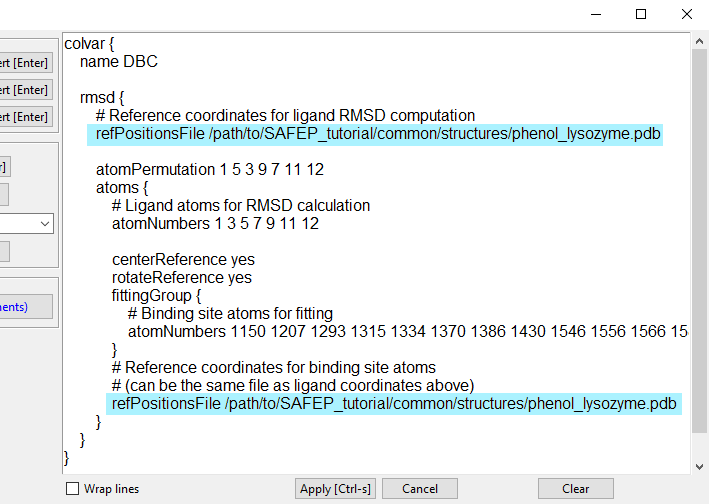
\includegraphics[width=0.75\linewidth ]{CV_dashboard_StepA.png} \label{fig:refposfiles}
            \end{itemize}
            \item \textbf{Save your edits:}\\
            Click the \button{Apply [Ctrl-s]} button.
        \end{enumerate}
        
        
        \item \textbf{Impose a restraint based on the DBC coordinate}
        \begin{enumerate}[label=\alph*., ref=\theenumi.\alph*]
            \item \textbf{Determine the Upper Wall of the DBC restraint:}
            \begin{itemize}
                \item In the \menu{Plots and real-time visualizations} panel of the dashboard, click \button{Histogram}. 
                If you don't see such a button, you need to upgrade your VMD installation. See software requirements for more details.
                \item From the histogram, estimate the  the 95th percentile of the bound state's DBC coordinate. Use the cumulative distribution line graph as a guide. The value doesn't need to be precise.  We selected 1.5 Angstroms. See \ref{app:Symmetry} for more details.
                \item Write this value down; you will need it in the next step. 
            \end{itemize}
            \item \textbf{Impose a flat-bottom harmonic potential:}
            \label{step:createDBC}
            \begin{itemize}
                \item Open the \menu{Biases} tab on the Colvars Dashboard and click \button{New bias [Ctrl-n]} to create a new biasing potential.
                \item Delete the default text.
                \item From the \menu{bias templates:} drop-down menu select \option{harmonicWalls} and click \button{Insert [Enter]}.
                \item Modify the bias to match the following parameters: \\
                { \ttfamily
                \begin{tabular}{l l}
                    colvars & DBC\\
                    upperWalls & [the DBC's 95th percentile just identified]\\
                    forceConstant & 200 \\
                \end{tabular} }\\
                The force constant in this case is in units of kcal/(mol$\cdot$\AA{}$^2$). The strength of restraint should be neither so great that it causes instabilities nor so weak that it fails to cleanly separate the bound and unbound ensembles. %move to appendix? Where?
            \end{itemize}
            \item \textbf{Save your edits:}\\
            Click the \button{Apply [Ctrl-s]} button.
        \end{enumerate}
        \item \textbf{Save the Colvars configuration to a file}
        \begin{enumerate}[label=\alph*., ref=\theenumi.\alph*]
            \item \textbf{Click} \button{Save} \textbf{at the top of the dashboard}
            \item \textbf{Save your file to} \filepath{stepA\_create\_DBC/outputs/DBC\_restraint.colvars}\\
            Note that if you choose to use a different file name or path you will need to update the files in the next step with the new name.
        \end{enumerate}
    \end{enumerate}

\subsection{\hspace{-1em}: Decouple phenol from the protein via FEP}\label{step:proteinDecouple}
    \begin{tcolorbox}[colback=blue!5!white,colframe=blue!75!black]
    In this section we will calculate $\Delta G_\mathrm{site}^*$ by decoupling the ligand from the protein binding site (and all other contents of the simulation box) using alchemical FEP. This FEP calculation is often the slowest to converge because of the narrowness of the bound distribution; i.e. there are far fewer bound configurations than unbound which makes it more likely to sample high energy (unimportant) conformations during decoupling. 
    To overcome this challenge, we will maintain the ligand in the bound configuration relative to the protein by restraining the DBC coordinate as defined in the previous subsection.
    \end{tcolorbox}
    
    \noindent{\textbf{Required Input:}}  
    \begin{itemize}
        \item Structure file: \filepath{common/structures/phenol\_lysozyme.psf} 
        \item Coordinate file: \filepath{common/structures/phenol\_lysozyme.pdb}
        \item DBC restraint parameters: \filepath{stepA\_create\_DBC/outputs/DBC\_restraint.colvars}
        \item NAMD configuration file: \filepath{stepB\_alchemy\_site/inputs/run.namd}
    \end{itemize}
    \textbf{Essential Output:}
    \begin{itemize}
        \item FEP configuration file: \filepath{stepB\_alchemy\_site/outputs/alchemy\_site.pdb}
        \item FEP trajectory file: \filepath{stepB\_alchemy\_site/outputs/alchemy\_site.dcd}
        \item FEP output file: \filepath{stepB\_alchemy\_site/outputs/alchemy\_site.fepout}
    \end{itemize}
    
\noindent\textbf{Procedure:}
\begin{enumerate}
    \item \textbf{Specify which atoms will be decoupled using the pdb beta field}\label{step:makeFEPpdbSite} 
        \begin{enumerate}[label=\alph*., ref=\theenumi.\alph*]
            \item \textbf{Open VMD and load the psf and pdb files specified in ``Required Input''.}
            \item \textbf{Set and write beta values:}
            \begin{itemize}
                \item Open the Tk Console from the Extensions menu.
                \item Ensure that your Tk Console is in the correct directory:\\
                \textInput{cd stepB\_alchemy\_site/outputs}
                \item Set the beta value of all atoms to 0:\\
                \textInput{[atomselect top all] set beta 0}
                \item Set the beta values of the ligand atoms to -1 for decoupling:\\
                \textInput{[atomselect top "resname PHEN"] set beta -1}
                \item Save as a pdb file:\\
                \textInput{[atomselect top all] writepdb alchemy\_site.pdb}
            \end{itemize}
        \end{enumerate}

    \item \textbf{Perform the FEP simulation}\\
    We have provided a configuration file for this FEP run: \filepath{stepB\_alchemy\_site/inputs/run.namd}. See the in-line comments in that file and \ref{app:FEPparameters} for a detailed description of the settings relevant to running FEP in namd.
    \begin{enumerate}[label=\alph*., ref=\theenumi.\alph*]     
         \item \textbf{Run the decoupling FEP}:\\
         Enter the following in your terminal window:\\
            \textInput{cd stepB\_alchemy\_site/inputs/}\\
            \textInput{namd2 +p4 run.namd \&> alchemy\_site.log}
        \item \textbf{[Optional] Start Step C:}\\
        If you have access to more compute resources, you can continue on to Step C while this FEP calculation is running. \textbf{Don't forget to return to analyze these data once the simulation is complete.} 
    \end{enumerate}
    
    \item \textbf{Analyze the trajectory}

    
    \begin{enumerate}[label=\alph*., ref=\theenumi.\alph*] \label{step:analyzeSite}
        \item \textbf{Visually inspect the trajectory in VMD:}
        \begin{itemize}
            \item Open VMD.
            \item Load the .psf (\filepath{common/structures/phenol\_lysozyme.psf}) and .dcd file(s) from the outputs of stepB.
            \item Ensure that the ligand remains in a bound-like configuration for the duration of the simulation.
        \end{itemize}
        \item \textbf{Measure the restraint energy:} 
        \begin{itemize}
            \item Open the Colvars Dashboard.
            \item Click \button{Load} and import your DBC restraint file (\filepath{DBC\_restraint.colvars}).
            \item Open the \menu{biases} tab, select the DBC restraint, and click \button{Energy Timeline}.
            \item The restraint energy should remain near zero for several nanoseconds, then increase and reach a maximum in the second half of the simulation (when the ligand is fully decoupled). If this is not the case, see \ref{app:troubleshooting}.
        \end{itemize}
        \item \textbf{Calculate $\Delta G^*_{\mathrm{site}}$ in the Jupyter Notebook:} \label{step:opennotebook}
        \begin{itemize}
            \item Navigate back to the tutorial root directory.
            \item Begin a Jupyter session and open the notebook titled \filepath{SAFEP\_Tutorial\_Notebook.ipynb}.
            \item Follow the in-notebook prompts to parse your new fepout file  (\filepath{stepB\_alchemy\_site/output/AFEP2-02.fepout}). By default, we use the sample output. Be sure to update the paths as indicated in the notebook:\\ 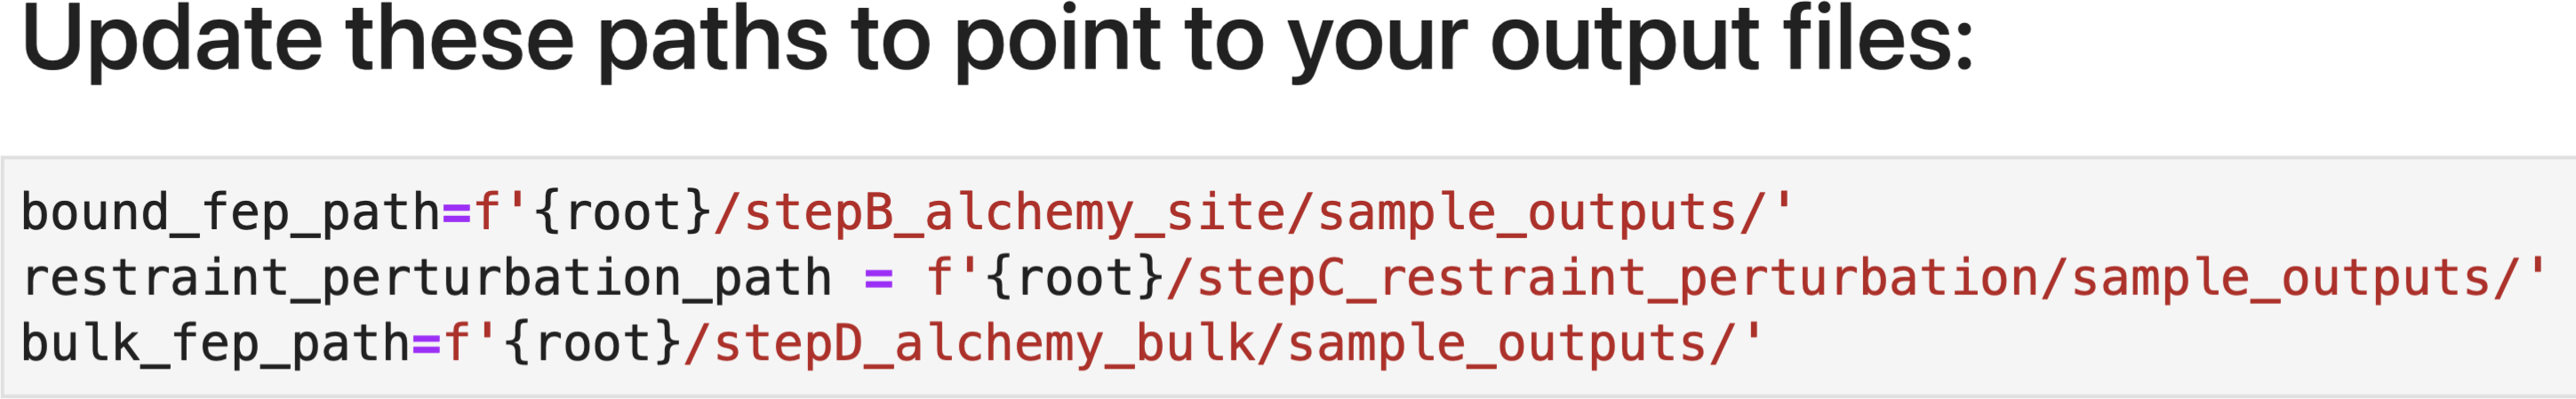
\includegraphics[width=0.75\textwidth, trim={0 0 0 2cm},clip]{update_paths.png}
            \label{fig:updatePaths}
            \item Compare your outputs to the sample outputs found in \ref{app:InterpretingFEP}.
        \end{itemize}
    \end{enumerate}
\end{enumerate}

\subsection{\hspace{-1em}: Compute the DBC restraint free energy correction}
\label{step:restraintPerturbation}
    \begin{tcolorbox}[colback=blue!5!white,colframe=blue!75!black]
    We designed the DBC restraint so that it doesn't do any significant work in the fully coupled system. However, it does reduce the entropy of the fully decoupled ligand, which would otherwise be exploring an ``empty'' simulation box. We need to calculate the corresponding free energy cost so we can correct for it. In this section we will use thermodynamic integration (TI) to calculate $\Delta \rm G_\mathrm{DBC}$; the free energy difference between a gas-phase ligand under DBC restraints {\textit vs} a (spherical) volumetric restraint. For more details see \ref{app:RFEP}.
    \end{tcolorbox}

 \noindent{\textbf{Required Input:}}  
    \begin{itemize}
        \item Structure file: \filepath{common/structures/phenol\_gas\_phase.psf} 
        \item Coordinate file: \filepath{common/structures/phenol\_gas\_phase.pdb}
        \item NAMD configuration file: \filepath{stepC\_restraint\_perturbation/inputs/run.namd}
    \end{itemize}
    \textbf{Essential Output:}
    \begin{itemize}
        \item Colvars configuration file: \filepath{stepC\_restraint\_perturbation/outputs/DBC\_Restraint\_RFEP.colvars}
        \item FEP trajectory file: \filepath{stepC\_restraint\_perturbation/outputs/RFEP.dcd}
        \item Colvars output file: \filepath{stepC\_restraint\_perturbation/outputs/RFEP.colvars.traj}
    \end{itemize}
    \textbf{Procedure:}

    \begin{enumerate}[label=\arabic*.]
    
        \item \textbf{Create coordinates upon which to base your restraints}
        \begin{enumerate}[label=\alph*., ref=\theenumi.\alph*]
            \item \textbf{Get set up:}
            \begin{itemize}
                \item Open VMD.
                \item Open the Tk Console.
                \item Open the Colvars Dashboard.
                
                \item \textbf{[Optional]} Extract the phenol from the phenol-lysozyme complex by running the following in the tkConsole. \textbf{Note: We have completed this step for you. The sample files can be found in \filepath{common/structures}.}
            
                \tkconsole{cd common/structures}
                
                \tkconsole{mol load psf phenol\_lysozyme.psf pdb phenol\_lysozyme.pdb}
                
                \tkconsole{set ligand [atomselect top "resname PHEN"]}
                
                \tkconsole{cd ../../stepC\_restraint\_perturbation/outputs}
                
                \tkconsole{\$ligand writepsf phenol\_gas\_phase.psf}
                
                \tkconsole{\$ligand writepdb phenol\_gas\_phase.pdb}

                \item Load \filepath{phenol\_gas\_phase.psf} and \filepath{phenol\_gas\_phase.pdb}

                \end{itemize}

            \item \textbf{Define the gas-phase spherical coordinate:} \label{step:defineGasRestraints}
            \begin{itemize}
                \item In the Colvars Dashboard, click \button{New [Ctrl-n]}.
                \item In the second line of the editor, replace the default name \textInput{myColvar} with \textInput{COM}.
                \item Delete \textInput{atomNumbers 1 2} and leave your cursor on that line.
                \item Using the \menu{Atoms from selection text:} tool in the left panel, enter \textInput{resname PHEN and noh} and click \button{Insert [Enter]}.
                \item Get the geometric center of the heavy atoms by  the following in the Tk Console:
                
                \textInput{measure center [atomselect top "resname PHEN and noh"]}
                
                \item Set the atoms of group 2 to \textInput{dummyAtom (x0, y0, z0)} where x0, y0, and z0 are the coordinates of the geometric center of the ligand you just retrieved in the previous step. Your editor should look similar to the figure below. Note the inclusion of commas in the \textInput{dummyAtom} statement.\\  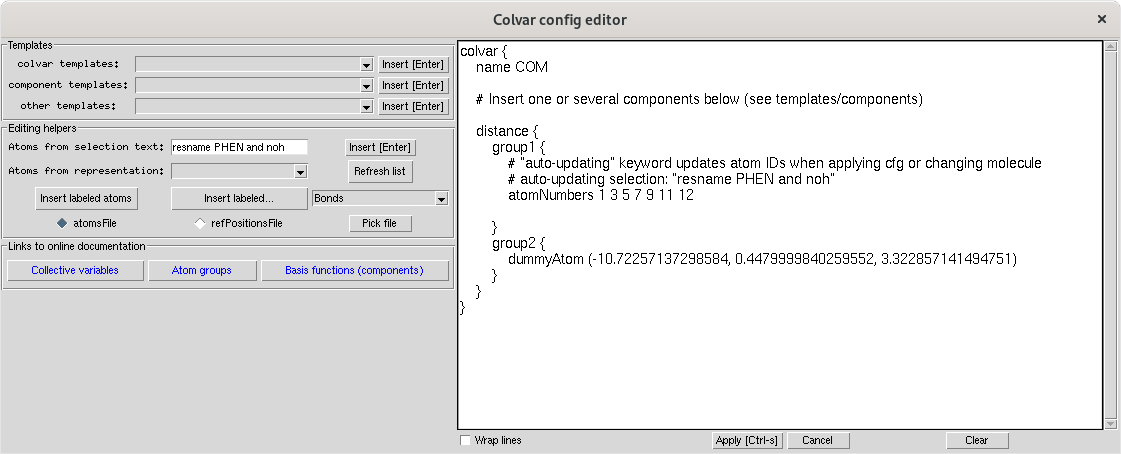
\includegraphics[trim={14cm 4cm 0 0}, clip, width=0.8\textwidth]{COM_restraint.png} \label{fig:COMtext}
                \item Save and close the colvar editor by clicking \button{Apply [Ctrl-s]}.
            \end{itemize}
            \item \textbf{Define the gas-phase DBC coordinate:} 
            \begin{itemize}
                \item Click \button{New [Ctrl-n]} again.
                \item In the second line of the editor, replace the default name \textInput{myColvar} with \textInput{DBC}.
                \item Delete the default distance component \textInput{distance\{...\}} and leave your cursor on that line.
                \item From the \menu{component templates} dropdown menu select \option{rmsd} and click \button{Insert [Enter]}.
                \item As before, add \textInput{atomPermutation 1 5 3 9 7 11 12} to the rmsd block to define the ligand symmetry.
                \item Delete \textInput{atomNumbers 1 2 3} and leave your cursor on that line.
                \item In the field labeled \menu{Atoms from selection text:} enter \textInput{resname PHEN and noh} and click \button{Insert [Enter]}. \label{step:setAtoms}
                \item Add \textInput{rotateReference off} and \textInput{centerReference off} to the \textInput{atoms} block.
                \item Replace the default \textInput{refPositionsFile @} line using the \option{$\circ$ refPositionsFile} radio button and the \button{Pick file} button to select \filepath{phenol\_gas\_phase.pdb}.
                \item Save and close the colvar editor by clicking \button{Apply [Ctrl-s]}.
            \end{itemize}
        \end{enumerate}
        \item \textbf{Define the restraints}
        \begin{enumerate}[label=\alph*., ref=\theenumi.\alph*]
            \item \textbf{Create the spherical restraint:}
            \label{step:createSpher}
            \begin{itemize}
                \item In the \menu{biases} tab of the Colvars Dashboard, click \button{New bias (Ctrl-n)} and delete the default text.
                \item From the \menu{bias templates} dropdown menu, select \option{harmonic walls} and press \button{Insert [Enter]}.
                \item Recall the upperWalls value you used for the DBC restraint in subsection \ref{step:createDBC} from Step A. You will need this value in this and the next step.
                \item Modify the bias to match the following parameters (see \ref{app:RFEP}):\\
                { \ttfamily
                \begin{tabular}{l l}
                    name & distance\_restraint\\
                    colvars & COM\\
                    outputEnergy & on\\
                    upperWalls & [DBC upperWalls plus 1]\\
                    forceConstant & 200\\
                \end{tabular} }
                

                \item Save and close the bias editor by clicking \button{Apply [Ctrl-s]}.
            \end{itemize}

            \item \textbf{Save the config file:}
            \begin{itemize}
                \item Click the \button{Save} button on the Colvars Dashboard.
                \item Save the file as \filepath{stepC\_restraint\_perturbation/outputs/DBC\_restraint\_RFEP.colvars}.
            \end{itemize}
        \item \textbf{Create a DBC restraint that gradually releases:} 
            \begin{itemize}
            \item We will use the provided setTI Tcl procedure.
            \item Open stepC\_restraint\_perturbation/inputs/run.namd in a text editor
            \item Find the block labeled ``COLVARS''
            \item Edit the input variables to match the following\\
            { \ttfamily
            \begin{tabular}{l l}
                cvName & DBC\\
                biasType & harmonicWalls\\
                upperWalls & [DBC upperWalls as determined in step A]\\
                targetForceConstant & 200.0\\
                forceConstant & 0.0\\
                targetForceExponent & 6.0\\
                targetEquilSteps & 500\\
                targetNumSteps & 300000\\
                nWindows & 40\\
                releaseFlag & True
            \end{tabular} }
            \end{itemize}
        \end{enumerate}
        
        \item \textbf{Run the TI simulation} 
        \begin{enumerate}[label=\alph*., ref=\theenumi.\alph*]
            \item \textbf{Enter the following in your terminal:}\\
            \textInput{cd stepC\_restraint\_perturbation/inputs}\\
            \textInput{namd2 +p1 run.namd \&> DBC\_FreeEnergy.log}
            \item \textbf{[Optional] Start Step D:}\\
            If you have access to more compute resources, you can continue on to Step D while the TI calculation is running.\\
            \textbf{Don't forget to return to analyze these data once the simulation is complete.}
        \end{enumerate}
        \item \textbf{Analyze the output} \label{step:analyzeRFEP}
        If any of these checks fails, check the Troubleshooting section of the Appendices (\ref{app:troubleshooting}).
        \begin{enumerate}[label=\alph*., ref=\theenumi.\alph*]
            \item \textbf{Visually inspect the trajectory in VMD:}
            \begin{itemize}
                \item Open VMD.
                \item Load the .psf, .pdb, and .dcd files associated with this tutorial step.
                \item The ligand should initially fluctuate roughly in place at the start and gradually explore the COM restraint space as the DBC restraint is released. 
            \end{itemize}
            \item \textbf{Check the collective variable trajectories:}
            \begin{itemize}
                \item Open the Colvars Dashboard
                \item Click \button{Load} and open the Colvars configuration file \filepath{DBC\_restraint\_RFEP.colvars}
                \item Select both the COM and DBC restraints
                \item Click \button{Timeline plot}
                \item Both coordinates should start low and gradually increase. The COM restraint should level out near its \textInput{upperWalls} restraint as shown: 
                
                \center{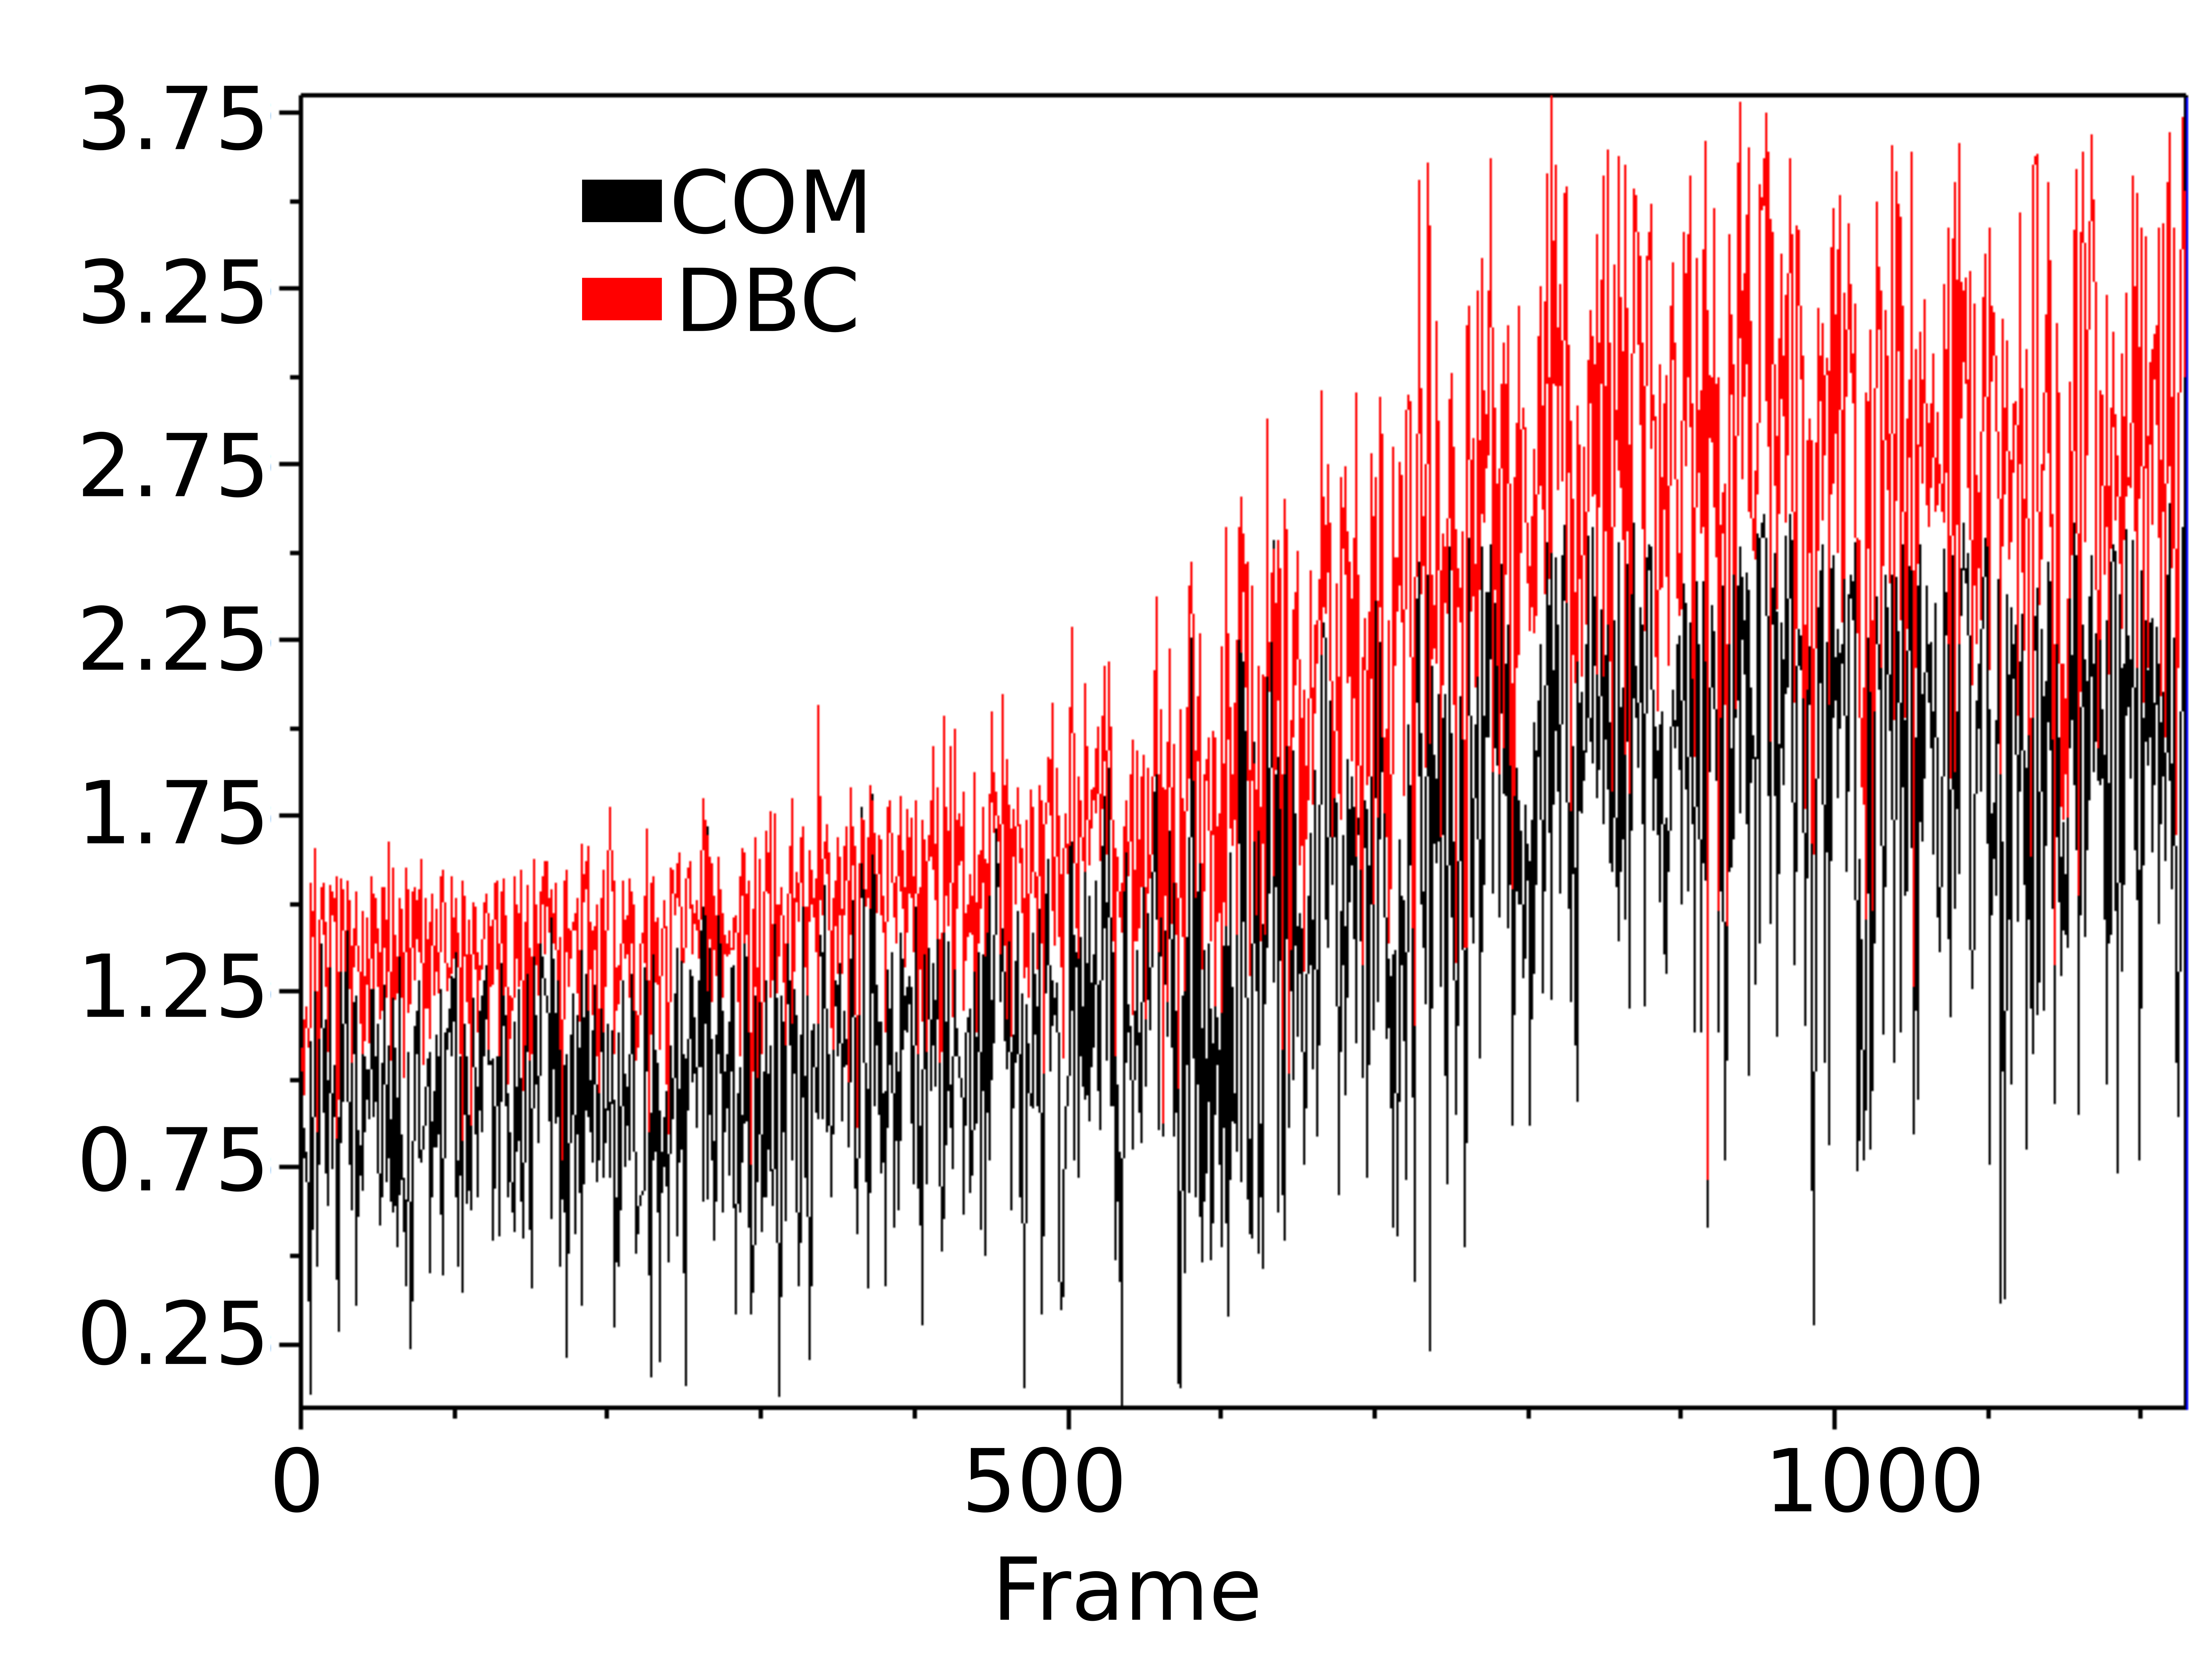
\includegraphics[width=0.5\linewidth]{sample_TI_traj.png}}
            \end{itemize}
            \item \textbf{Calculate the $\Delta G_\mathrm{DBC}$ in the Jupyter Notebook:}
            \begin{itemize}
                \item Open the Jupyter Notebook as in subsection \ref{step:opennotebook} from step B. Update the paths in ``User Settings'' as needed. Remember, sample data will be used by default.
                \item Run the first several cells at least until the first FEP analysis section. 
                \item Run the first cell in the section titled ``Process the DBC TI calculation'' and make sure the DBC and COM walls are correct.
                \item Run all the cells in that section. Sample outputs and more details can be found in \ref{app:RFEP}
                \item The output will include the $\Delta G_\mathrm{DBC}$ in kcal/mol as well as an error estimate based on the analytical derivative of the free energy with respect to lambda. See the colvars documentation for more details.
            \end{itemize}
        \end{enumerate}
    \end{enumerate}
    
\subsection{\hspace{-1em}: Decouple phenol from bulk solvent}

\label{step:bulkDecoupling}
    \begin{tcolorbox}[colback=blue!5!white,colframe=blue!75!black]
    You have completed one alchemical FEP calculation already, but double-decoupling methods require two such calculations to close the thermodynamic cycle. We need to know the free energy of transferring the ligand from the binding site into vacuum, {\it and} from vacuum into the bulk.  In this section we will calculate the latter term, $\Delta G_\mathrm{bulk}^*$, by decoupling the ligand from the bulk solution. 
    \end{tcolorbox}
\noindent{\textbf{Required Input:}}  
    \begin{itemize}
        \item Structure file: \filepath{common/structures/phenol\_water.psf} 
        \item Coordinate file: \filepath{common/structures/phenol\_water.pdb}
        \item NAMD configuration file: \filepath{stepD\_alchemy\_bulk/inputs/run.namd}
    \end{itemize}
    \textbf{Essential Output:}
    \begin{itemize}
        \item FEP configuration file: \filepath{stepD\_alchemy\_bulk/outputs/alchemy\_bulk.pdb}
        \item FEP trajectory file: \filepath{stepD\_alchemy\_bulk/outputs/alchemy\_bulk.dcd}
        \item FEP output file: \filepath{stepD\_alchemy\_bulk/outputs/alchemy\_bulk.fepout}
    \end{itemize}
    \textbf{Procedure:}
    \begin{enumerate}
    \setcounter{enumi}{-1}
        \item \textbf{Prepare the ligand as you would for traditional FEP.} Use a conservative box size; very small boxes are more prone to instabilities and self-interactions which will lead to artifacts in the final free energy estimate. \textbf{Note: this step has been completed for you.}
        \item \textbf{Specify which atoms will be decoupled using the pdb beta field}\label{step:makeFEPpdb} 
        \begin{enumerate}[label=\alph*., ref=\theenumi.\alph*]
            \item \textbf{Open VMD and load the psf and pdb files specified in ``Required Input''.}
            \item \textbf{Set and write beta values:}
            \begin{itemize}
                \item Open the Tk Console
                \item Ensure that your Tk Console is in the correct directory:\\
                \textInput{cd stepD\_alchemy\_bulk/outputs}
                \item Set the beta value of all atoms to 0:\\
                \textInput{[atomselect top all] set beta 0}
                \item Set the beta values of the ligand atoms to -1 for decoupling:\\
                \textInput{[atomselect top "resname PHEN"] set beta -1}
                \item Save as a pdb file:\\
                \textInput{[atomselect top all] writepdb alchemy\_bulk.pdb}
            \end{itemize}
        \end{enumerate}

        \item \textbf{Run the ligand decoupling simulation in bulk solvent}\\
        \textInput{cd stepD\_alchemy\_bulk/inputs}\\
        \textInput{namd2 +p4 run.namd \&> alchemy\_bulk.log}

        \item \textbf{Analyze the output} \label{step:analyzeBulk}
        \begin{enumerate}[label=\alph*., ref=\theenumi.\alph*]
            \item \textbf{Visually inspect the trajectory in VMD:}
            \begin{itemize}
                \item Open VMD.
                \item Load the .psf, .pdb, and .dcd files associated with your simulation.
                \item The ligand should diffuse normally at the start of the simulation but behave more and more like a gas-phase molecule.
            \end{itemize}
            \item \textbf{Calculate $\Delta G^*_\mathrm{bulk}$ in the Jupyter Notebook}
            \begin{itemize}
                \item Open the Jupyter Notebook as in subsection \ref{step:opennotebook} from Step B.
                \item Confirm that \textInput{bulk\_fep\_path} points to your files
                \item Parse the \filepath{.fepout} file by running all the cells in the Jupyter notebook section titled ``Decoupling from Solvent''.
            \end{itemize}

        \end{enumerate}

    \end{enumerate}

\subsection{\hspace{-1em}: Calculate corrections and combine quantities}\label{step:combinequantities}
    \begin{tcolorbox}[colback=blue!5!white,colframe=blue!75!black]
    We will now calculate $\Delta G^\circ_\mathrm{V}$ analytically. With this final piece of information, we can calculate the dissociation constant and estimate a titration curve based on the probability of occupancy assuming a two-state system: $P_\mathrm{bind}=\frac{[PHEN]}{K_\mathrm{d}+[PHEN]}$ where the dissociation constant, ${K_\mathrm{d}}=e^{\left(\beta \Delta G^\circ_\mathrm{bind}\right)}$. For additional information see \ref{app:bindingProbability}.
    \end{tcolorbox}
\noindent{\textbf{Required Input:}}  
    \begin{itemize}
        \item Site FEP data: \filepath{stepB\_alchemy\_site/outputs/alchemy\_site.fepout} 
        \item Restraint perturbation data (RFEP/TI): \filepath{stepC\_restraint\_perturbation/outputs/RFEP.colvars.traj}
        \item Bulk FEP data: \filepath{stepD\_alchemy\_bulk/outputs/alchemy\_bulk.fepout}
    \end{itemize}
    \textbf{Essential Output:}
    \begin{itemize}
        \item $\Delta G^\circ_{\mathrm{bind}}$
        \item \filepath{titration\_curve.pdf}
    \end{itemize}
    \textbf{Procedure:}
    \begin{enumerate}
    \item Complete any unfinished analyses in previous steps (i.e. steps \hyperref[step:analyzeSite]{B.\ref{step:analyzeSite}}, \hyperref[step:analyzeRFEP]{C.\ref{step:analyzeRFEP}}, and \hyperref[step:analyzeBulk]{D.\ref{step:analyzeBulk}}).
    It is especially important to examine the trajectories since numerically subtle biases are more obvious from the trajectory.
    \item Open the Jupyter notebook and navigate to the section labeled ``Volumetric Restraint Contribution''.
    \item Run the section to calculate the volumetric free energy contribution.\label{step:dGV}
    See \ref{app:COMCorrection} for a more detailed explanation.\\
    \textbf{Note:} At this point you will either need to have completed all simulations or use the sample data provided. To use the sample data, change the path variables (\textInput{bound\_fep\_path},\textInput{ restraint\_perturbation\_path}, and \textInput{bulk\_fep\_path\textrm{)}} to use the files in their respective \filepath{./sample\_outputs} directories. 
    \item Calculate the overall $\Delta G_\mathrm{bind}^\circ$ and compute a titration curve by running the cells in the section ``Binding Free Energy''.
    \item Compare your final $\Delta G_\mathrm{bind}^\circ$ to the literature value of -5.44 kJ/mol\cite{Merski2013}.
    \item Compare your titration curve to Figure~\ref{fig:titrationCurve} below.
\end{enumerate}
\begin{figure}[!htb]
    \centering
    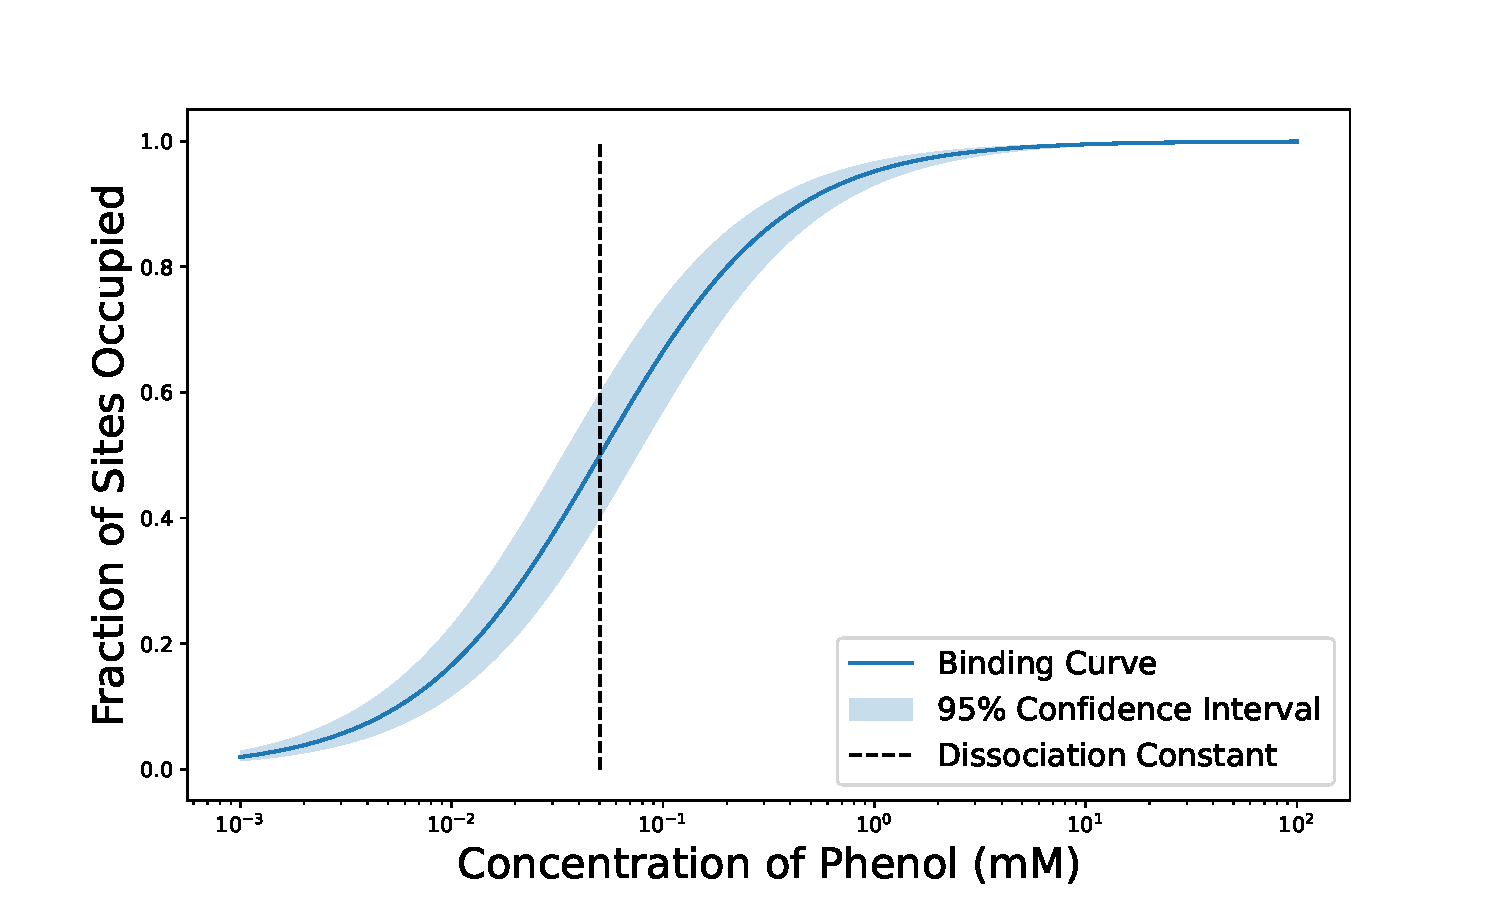
\includegraphics[width=0.5\textwidth]{titration_curve}
    \caption{\textbf{An example titration curve} generated using Equation \ref{eq:bindingStatmech}. The 95\% confidence interval is generated by $\pm 1.96*\rm SEM$ of the $\Delta G_\mathrm{bind}$}
    \label{fig:titrationCurve}  
\end{figure}


\twocolumn
\begin{table}[H]
    \centering
    \caption{Symbols used in this tutorial.}
    \label{tab:variables}
    \begin{tabular}{  p{.26\linewidth} | p{.7\linewidth}  }
        \textbf{Symbol} & \textbf{Definition}\\
        \hline
        $d$ & Distance-to-Bound-Configuration (DBC) \\
        \hline
        $\Delta G^\circ_\mathrm{bind}$ & Standard free energy of binding\\
        \hline 
        $\Delta G^*_\mathrm{bulk}$ & Free energy of decoupling the ligand from the bulk solution \\
        \hline 
        $\Delta G_\mathrm{DBC}$ & Free energy of imposing the DBC restraint on the ligand from a COM restraint \\
        \hline
        $\Delta G^*_\mathrm{site}$ & Free energy of decoupling the ligand from the binding site \\
        \hline 
        $\Delta G^\circ_\mathrm{V}$ & Free energy of releasing the ligand to the standard state from the Center of Mass restraint\\
        \hline 
        $k$ & A force constant for a restraint\\
        \hline
        $k_\lambda$ & A force constant that is a function of $\lambda$\\
        \hline
        $k_0$ and $k_1$ & Force constants when $\lambda=0$ and $\lambda=1$, respectively\\
        \hline
        $L$ and $L^\prime$ & Arbitrary ligand concentrations\\
        \hline
        $m$ & Number of non-decoupled ligands in the bulk system\\
        \hline
        $p_\mathrm{occ}$ and $p_\mathrm{unocc}$ & The probability of a site being occupied or unoccupied, respectively\\
        \hline
        $r$ & Center Of Mass (COM) displacement\\
        \hline
        $r_R$ & Upper wall of a COM restraint\\
        \hline
        $U_\mathrm{FW}$ & Energy function of a flat-well potential\\
        \hline
        $V$ & Volume of the bulk system\\
        \hline
        $V_R$ & Volume of a sphere with radius $r_R$\\
        \hline
        $Z_\mathrm{occ}$ and $Z_\mathrm{unocc}$ & Partition functions for the occupied state and unoccupied state, respectively\\
        \hline
        $\alpha$ & An exponential smoothing parameter\\
        \hline
        $\beta$ & Thermodynamic beta with units of $\frac{kcal}{mol}$\\
        \hline
        $\Theta_i$ & DBC test function for a single ligand\\
        \hline
        $\Theta_\mathrm{occ}$ & Occupancy test function for a single binding site\\
        \hline
        $\lambda$ & A coupling parameter $\lambda\in\{0,1\}$\\
        \hline
        $\xi$ & An arbitrary collective variable\\
        \hline
        $\xi_\mathrm{max}$ & Upper wall of a flat-well restraint on $\xi$\\
    \end{tabular}
\end{table}

%\appendix
%\label{appendices}
\counterwithout{figure}{section}
\setcounter{section}{0}
\renewcommand\thesection{Appendix~\Alph{section}}
\renewcommand\thesubsection{\thesection.\arabic{subsection}}



\section{System Selection and Setup}
\label{app:motivation}
Lysozyme L99A/M102H (PDBid 4I7L) was chosen for several reasons. Lysozyme L99A/M102H is a small protein that binds a small, rigid molecule with reasonably high affinity which has already been measured experimentally. These properties make it well-suited as a model for prototyping and validating free energy calculation methods generally. 

Because lysozyme is elongated, we save some computation time by using a narrower box. We avoid self-interactions by imposing a soft harmonic restraint on the protein's alpha carbons provided in \filepath{common/protein\_tilt.colvars}. \label{app:equilibration}
The provided systems were prepared using CHARMM-GUI\cite{Jo2008, Lee2016} using a truncated lysozyme (PDBid 4I7L, residues 3 to 157) and solvated using default parameters (TIP3P water, 0.15M NaCl). 
The production run uses largely default parameters and settings. The only notable exception is that \textInput{WrapAll} should be set to \textInput{off}. 
This is because wrapping across the PBC can cause unexpected results during analysis which can compromise the FEP and TI calculations.

\section{Running FEP in NAMD}\label{app:FEPparameters}
\subsection{Configuration Files}
In addition to the configuration, forcefield, and structural files, running FEP in NAMD requires a particular pdb file (sometimes called a ``fep file'') that contains flags that indicate which atoms are being coupled or decoupled. This is usually indicated in the beta column as '-1' for decoupling or '1' for coupling. All other beta fields should be 0.

The configuration file also contains some additional options that are detailed in the NAMD user guide \cite{Bernardi2020} and described briefly in the provided configuration files. While most of the settings should remain unchanged in a wide range of settings, there are a few exceptions.

\textbf{\textInput{alchOutFreq}} determines the number of steps between collecting FEP samples. It should be set to a multiple of \textInput{fullElectFreq} to ensure accurate energy estimates. Later versions of NAMD should resolve this issue automatically, see \href{https://www.ks.uiuc.edu/Research/namd/mailing_list/namd-l.2020-2021/1487.html}{Bug advisory and Workaround}. Additionally the sampling frequency should be between 50 and 200 steps; sampling too frequently will result in bloated data sets of highly autocorrelated samples while sampling infrequently will result in too few samples to get a well-converged estimate of the change in free energy.

\textbf{\textInput{alchVdwShiftCoeff}} controls the strength of the soft-core potential which is essential to prevent “end-point catastrophes” in which one or more Lennard-Jones potentials diverge to infinity near lambda=0 or lambda=1. Higher values result in ``softer'' potentials but can introduce artifacts. For this reason, the \textInput{alchVdwShiftCoeff} should be kept between 5 and 8. See \cite{Zacharias1994} and \cite{Ebrahimi2022} for more details.

\textbf{\textInput{alchEquilSteps}} hard-codes the time between starting a new lambda value and beginning to sample the ensemble. Alchemlyb and PymBAR provide functions that will down-sample the data set using automated equilibration and autocorrelation detection schemes. We have found that automated equilibrium detection performs about as well as manually setting \textInput{alchEquilSteps} and autocorrelation is the bigger problem when trying to assess convergence. See \cite{shirts2008statistically} for a more detailed discussion of equilibrium detection, autocorrelation, and their effects on free energy estimation. See \ref{app:InterpretingFEP} or the provided Jupyter notebook for more information on how these are applied to analysis.

\textbf{\textInput{deltaLambda}} is passed as a parameter to the runFEP function and determines the width of the lambda windows. Narrower windows will converge faster but will increase the total number of windows required to span $\lambda=0$ to $\lambda=1$. 
As a result, we need to empirically optimize the number and length of windows. 
See \ref{app:InterpretingFEP} and \ref{app:troubleshooting} for more details on assessing and optimizing these parameters. 
The number and length of windows used here ($\sim$ 40~ns total simulation time) are a good starting point, but we have used as much as 400~ns for very flexible ligands in superficial binding sites\cite{Petroff2022}.

\textbf{\textInput{IDWS}} (interleaved double-wide sampling) 
tells NAMD to alternate between sampling the forward and reverse lambda directions (via the runFEP function, which sets the \textInput{alchLambdaIDWS} parameter). This should be set to ``true'' thus removing the need for independent forward and backward runs. This is a rigorous approach because of the reversibility of the transformation. Note that this may cause some correlation between forward and backward samples depending on the value of \textInput{alchOutFreq}.

\subsection{Parsing and Data Analysis}\label{app:Analysis}
In this tutorial we have recommended using a Jupyter notebook for analysis. The first decision is whether or not to use Alchemlyb's equilibrium detection. In our experience it has made very little difference, but if you suspect poor equilibration it may be helpful. In the provided notebook, simply set \textInput{detectEQ} to \textInput{True} before reading in any data.

After initial reading and parsing, you will see the estimated $\Delta G_\mathrm{site}^*$ with standard error in the section labeled ``Get $\Delta G$.'' We provide conservative settings which (though not the most efficient) should result in good convergence for this system. As noted in the previous section, more complicated systems with more internal degrees of freedom may require much longer sampling and narrower lambda windows. In such systems, it is not uncommon for errors to be as high as 0.5 or 1kcal/mol. Errors larger than 1kcal/mol often indicate poor convergence and are likely to suffer from other issues (e.g. hysteresis). See \ref{app:troubleshooting} for more information on how to identify and resolve the underlying causes.

\subsection{Interpreting the Figures}\label{app:InterpretingFEP}
In this section we describe the contents and meaning of each of the figures generated by the provided Jupyter notebook. See \ref{app:troubleshooting} for strategies to address discrepancies between your own results and those described here. An example of a well-converged calculation is shown in Figure ~\ref{fig:FEPexample}.

Cumulative and per-window $\Delta G$ curves (first and second panels of Figure~\ref{fig:FEPexample}) should be reasonably smooth. For typical lambda windows (1 to 3~ns), the magnitude of the $\Delta G$ should be less than a few kcal/mol per window. Sharp cusps and large jumps (especially near lambda 0.5) often indicate either insufficient samples or too-wide lambda windows.

\begin{figure}[!ht]
    \centering
    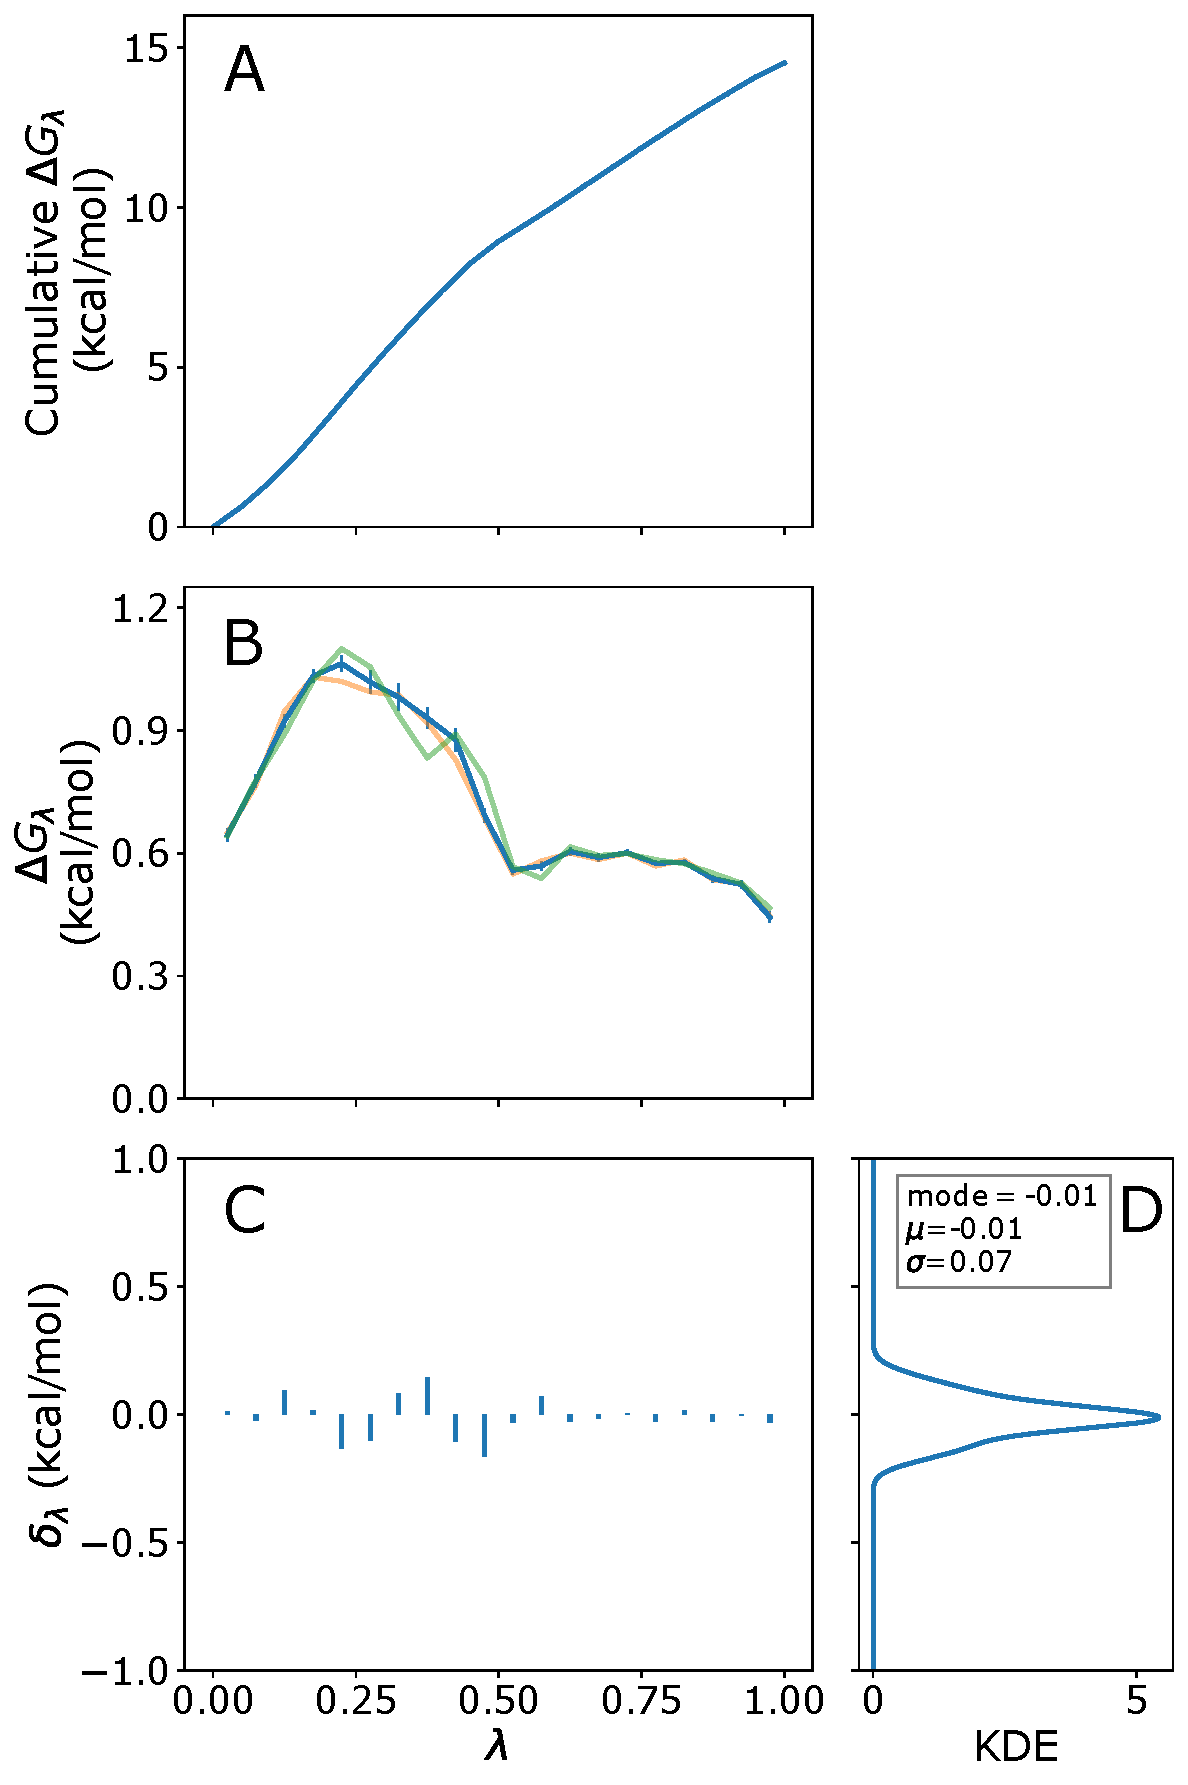
\includegraphics[width=0.9\linewidth]{bound_generalFigures}
    \caption{\textbf{Example results from protein-phenol decoupling calculation.} The first panel shows the cumulative change in free energy with accumulated error. The second panel shows per-window difference in free energy ($\Delta G_\lambda$) calculated by the BAR estimator (blue), and exponential estimators for forward (orange) and backward (green) samples. The third and fourth panels show the hysteresis ($\delta_\lambda$) and its probability density function estimated by kernel density estimation (KDE), respectively. Error bars indicate standard error of the mean; cumulative (first panel) or per-window (second and third panels).
    }\label{fig:FEPexample}
\end{figure}

The $\delta_\lambda$ plots (third and fourth panels of Figure~\ref{fig:FEPexample}) are used to diagnose hysteresis with respect to lambda. No value should be more than about 1~kcal/mol with a mean close to zero and an absolute skewness less than 0.5. Failure to meet any of these criteria indicates that one or more of the lambda windows has not, in fact, reached equilibrium or converged.

Finally, the convergence plot should display two curves that meet quickly (before 0.5), and both curves should level out well before 1 like the example shown in Figure~\ref{fig:convergenceExample}. If they are still changing at 1 or have not gotten to within 0.5~kcal/mol by $\lambda=0.5$, the system is unlikely to be converged at one or more lambda values and the final $\Delta G$ estimate is likely to be inaccurate.

\begin{figure}[htb]
    \centering
    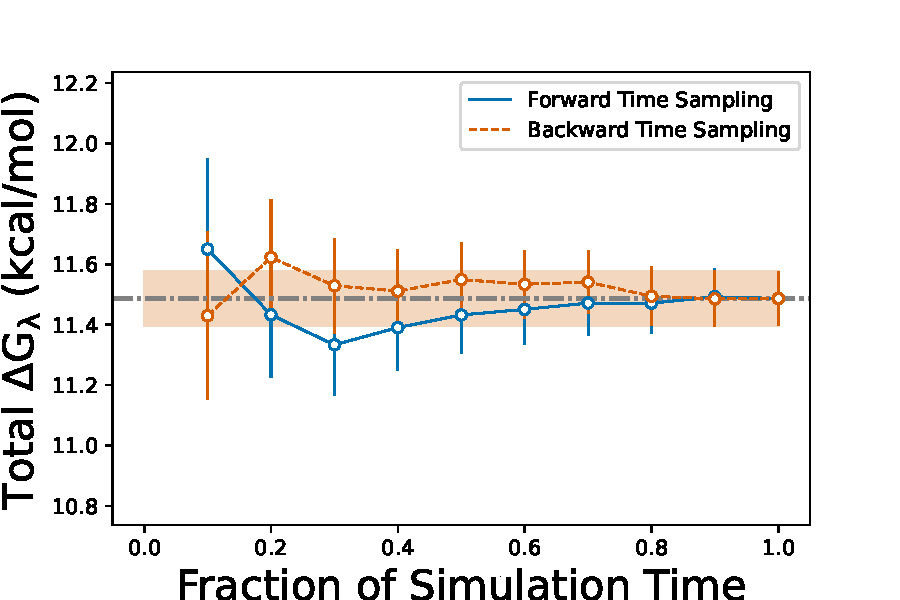
\includegraphics[width=250pt]{good_convergence}
    \caption{\textbf{Example convergence data.} We believe this calculation is well-converged due to the overlap near the half-way point and the leveling out of both curves well before the end. Error bars indicate standard error of the mean.
    }\label{fig:convergenceExample}
\end{figure}

\section{Restraints}\label{app:restraints}
In the simulation where the ligand is decoupled from the site, restraints that keep the ligand from diffusing away must be applied. This serves two purposes:\cite{Hermans1986} first, it ensures that the long-time results of the free energy computation describe what we want, which is decoupling from the bound state; second, it accelerates convergence of the computation by limiting the space to be sampled.
Thus binding restraints are essential both for estimating a well-defined free energy of binding, and for minimizing the statistical noise on that estimate.
This is often achieved by layering several rotation and translational restraints on the ligand. \cite{Hermans1997, Gilson1997, Boresch2003, Hamelberg2004, Woo2005, Deng2006}.
The main draw-back of such approaches is that each restraint must be designed and parameterized which adds to 1) the time and effort required to setup the simulations and 2) the complexity of the simulations themselves.
As a result, troubleshooting and interpretation are more difficult and time-consuming.
SAFEP, in contrast, uses just one restraint, the distance-to-bound-configuration (DBC), which is both robust and requires minimal parameterization \cite{Salari2018}.

\subsection{Flat-well Restraints}

An ideal restraint for decoupling simulations would precisely separate the bound and unbound ensembles without modifying either. That is, it would be of the form:
\begin{equation} \label{eq:squareWell}
    U(\xi) = \begin{cases}
        0 &, \; \xi\; \text{in the bound state}\\
        \infty &, \; \text{otherwise}
    \end{cases}
\end{equation}
\noindent This singular potential, however, would create numerical instability in a molecular dynamics simulations. We, therefore, impose smoothed flat-well restraints which result in finite restorative forces when the system crosses the boundary between macrostates, but leave the target ensemble essentially unmodified. Such restraints approximate square wells with the form:
\begin{equation} \label{eq:harmonicWall}
    U_\mathrm{FW}(\xi) = \begin{cases}
        \frac{1}{2}k \left(\xi-\xi_\mathrm{max}\right)^2 &, \; \xi > \xi_\mathrm{max}\\
        0                                                & \; \text{otherwise}
    \end{cases}
\end{equation}

\subsection{The Distance-to-Bound Configuration (DBC) Coordinate}
\subsubsection{Definition of DBC}
The DBC is the root-mean-square deviation (RMSD) of a subset of ligand coordinates from a typical bound pose \textit{in the frame of reference of the binding site}.
In general, all heavy atoms can be included in the DBC, but larger, more flexible ligands may be better restrained using a narrower subset of atoms. 
This single, scalar coordinate captures any relative motion of the ligand with respect to the binding site as well as any conformational change of the ligand. 
To obtain a DBC restraint, we apply a flat-well potential defined by Equation~\ref{eq:harmonicWall} to a DBC coordinate.
See Ref.~\citenum{Salari2018} for details.
\begin{figure}[!htb]
    \centering
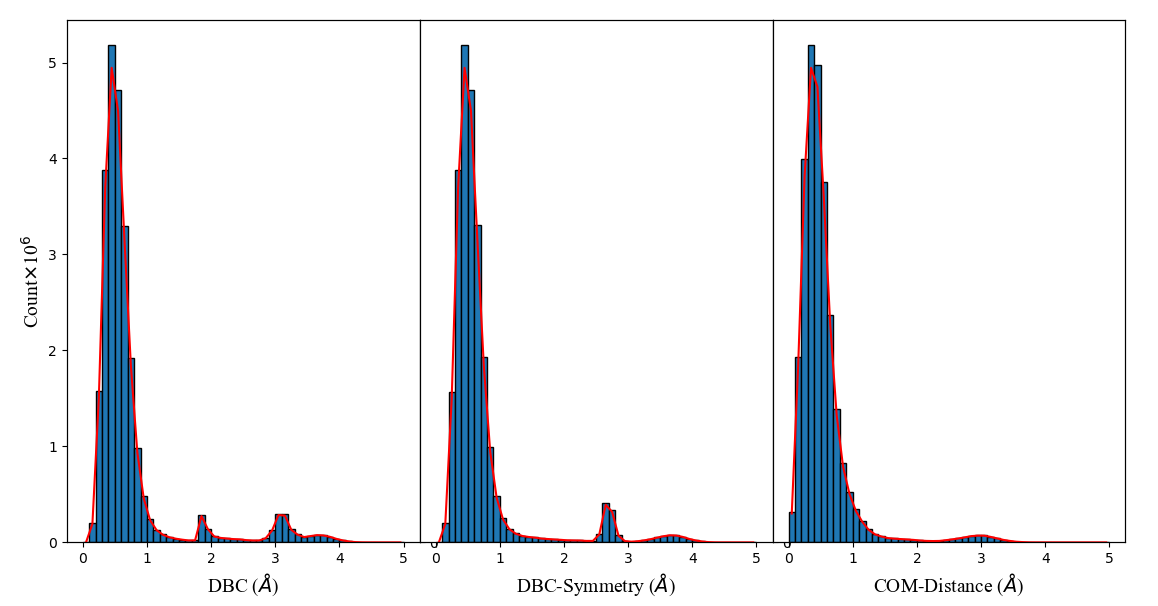
\includegraphics[width=0.4\textwidth]{histogram.png} 
    \caption{Screenshot from the Colvars Dashboard showing an example asymmetric DBC distribution from an unbiased simulation. If the phenol had flipped about the symmetric axis, there would be a second peak about 1.8~\AA{}}
\label{step:DBCwidth}
\end{figure}

\subsubsection{Symmetric DBC}
\label{app:Symmetry}

One peculiarity of the model system used here is that the ligand, phenol, is symmetric. 
Although this isn't strictly problematic, it does require a little extra accounting. 
Although this case lends itself well to an analytical solution (an extra term of $kT\ln 2$), a symmetric DBC is much more general and robust\cite{Ebrahimi2022}.
This is especially the case for very flexible ligands that would require much more complicated analytical corrections. The Colvars keyword \texttt{atomPermutation} can be used to define these symmetries:

\begin{enumerate}
     \item The easiest way to identify equivalent atoms is to label them.
     \item Use the \menu{Graphics$\rightarrow$Representations} interface to hide all atoms except the ligand.
     \item Use the labeling tool to label the four symmetric carbons as shown:
     \begin{center}
        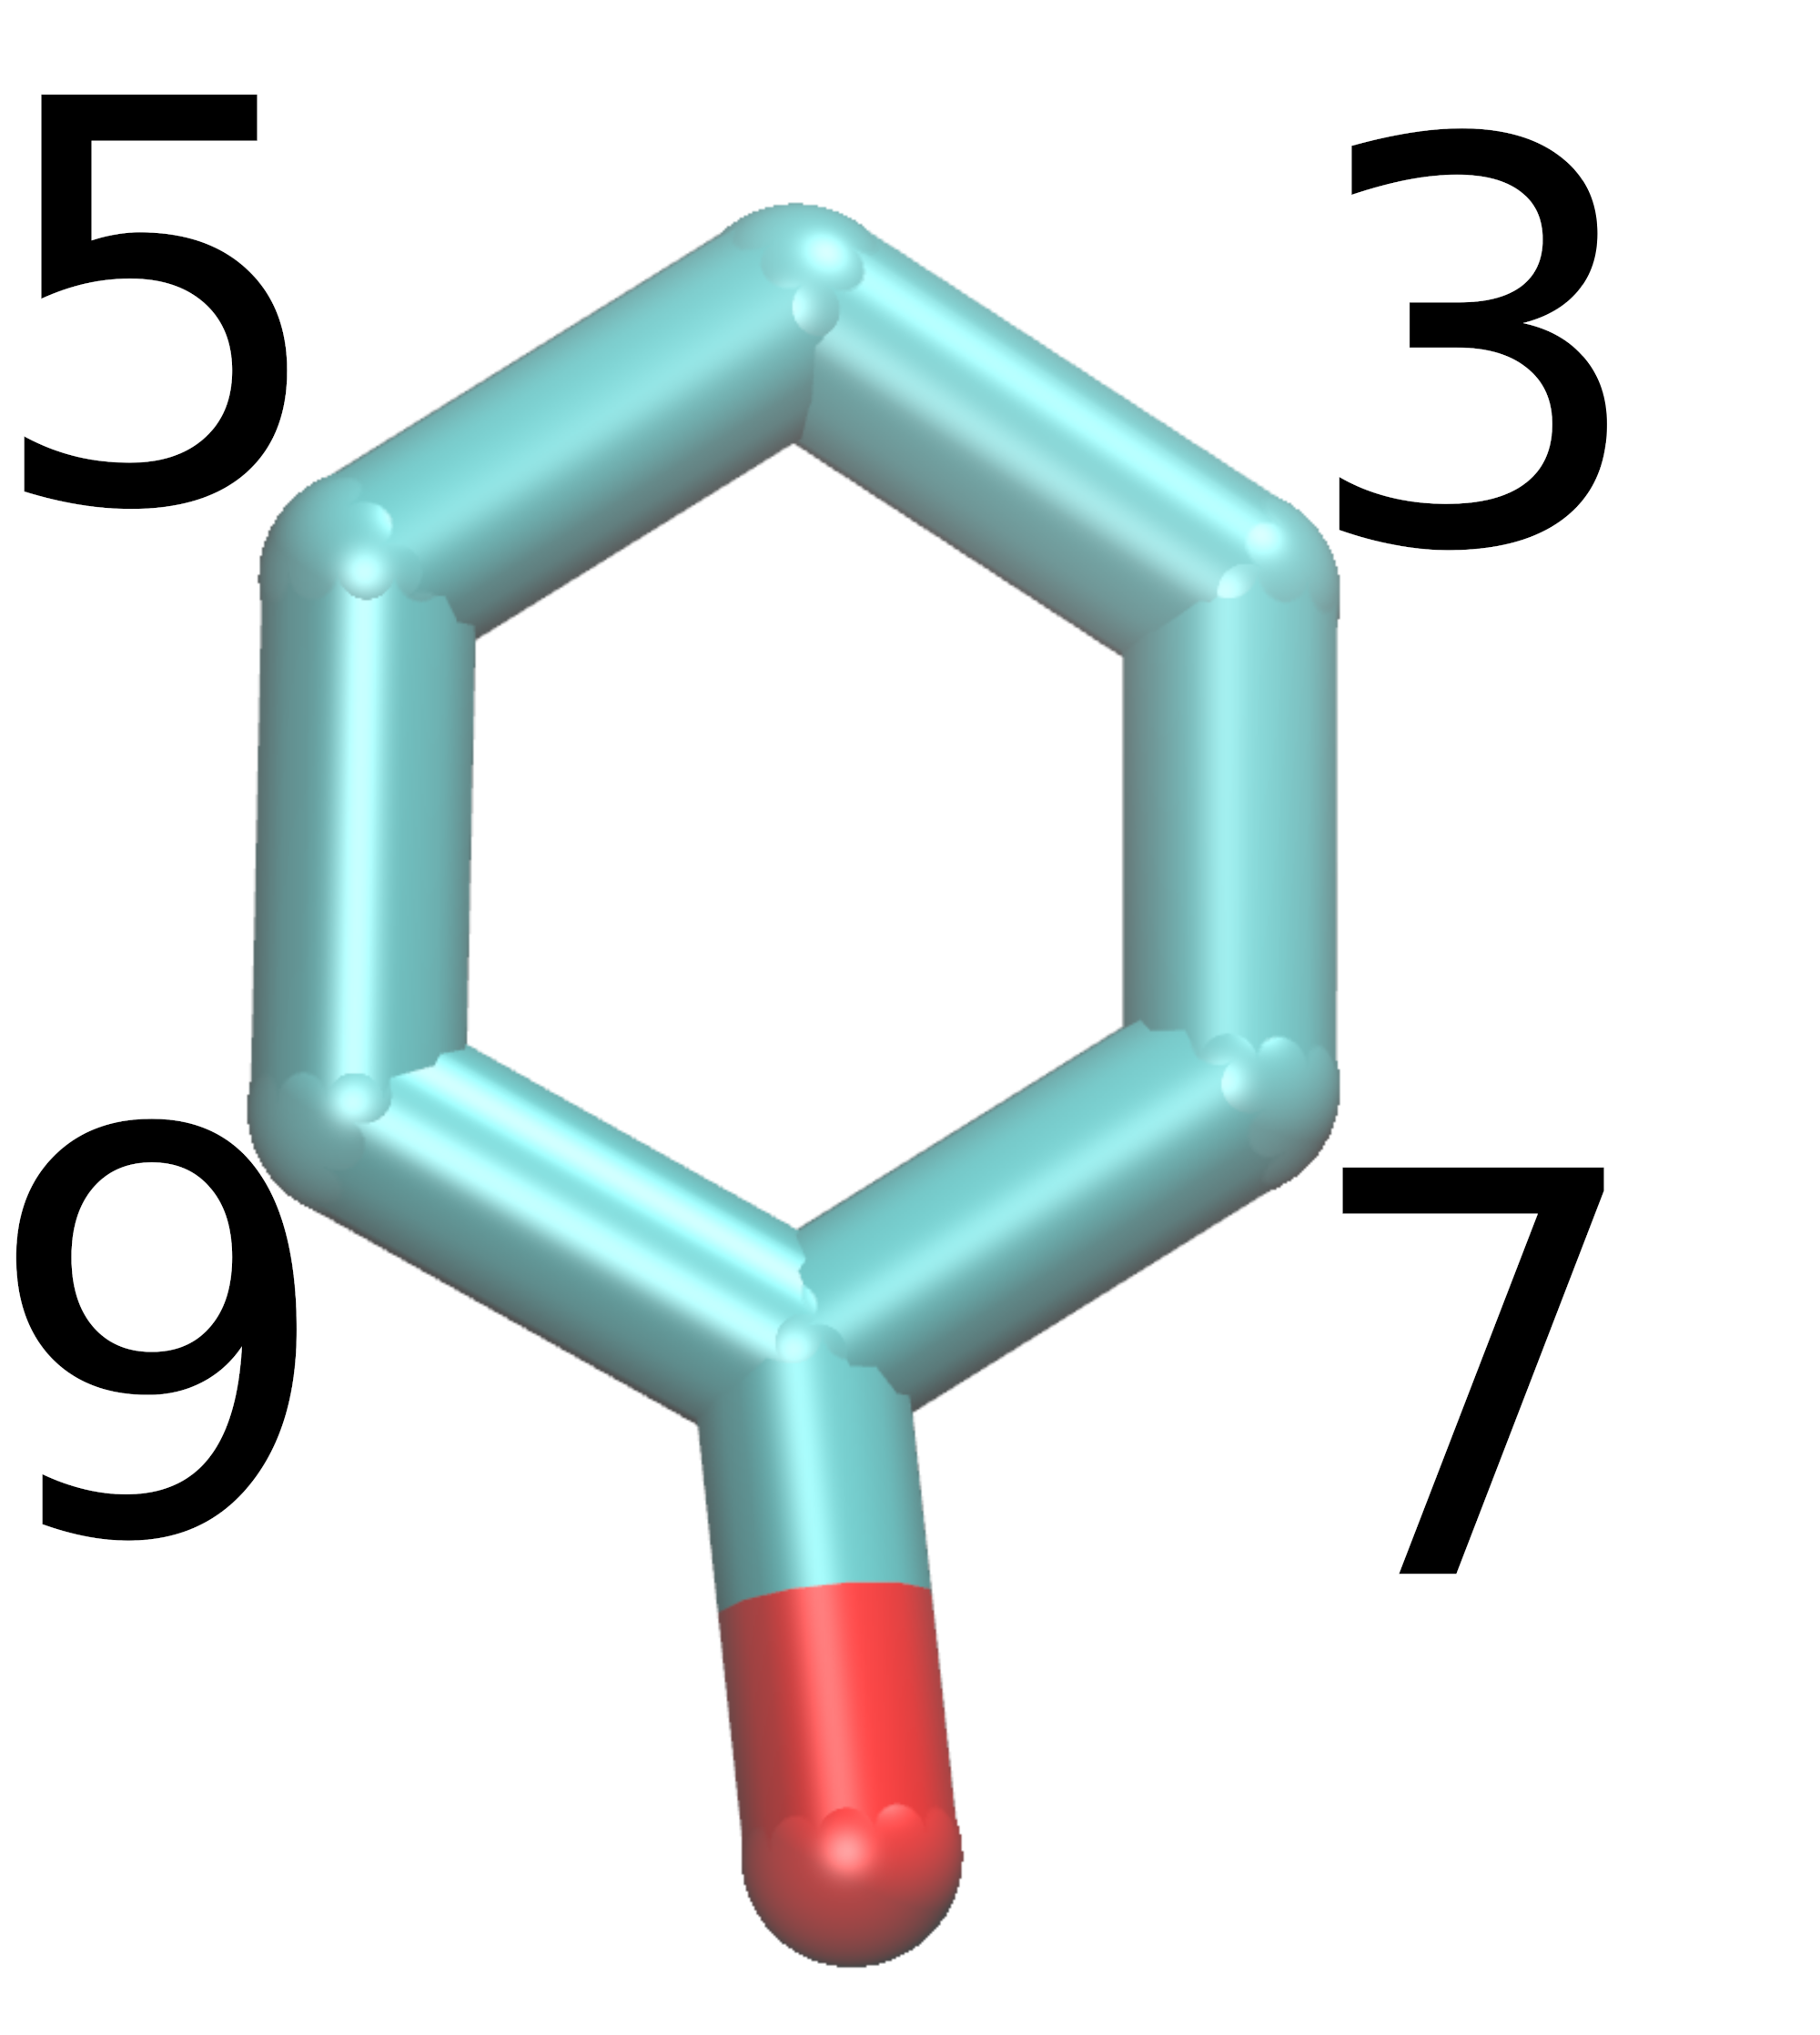
\includegraphics[width=0.2\linewidth]{example_symmetry_labels.png}
     \end{center}
     \item Open \menu{Graphics$\rightarrow$Labels...}.
     \item Select all four labels from the list by clicking and dragging
     \item Open the tab titled \menu{Properties} and change the format string to \textInput{\%1i}
     \item You may wish to adjust other settings in this menu to make the labels more visible
     \item Your view should now look something like the image above with the serial number of each atom indicated.
     \item In the Colvar config editor window, place your cursor on the line before \textInput{atoms \{} and add \textInput{atomPermutation \{11 7 3 1 5 9 12\}}
     \item Your console should now look like this:
    \begin{lstlisting}[language=tcl]
    colvar {
      name DBC_sym
      rmsd {
        atomPermutation {11 7 3 1 5 9 12}
        atoms {
          atomNumbers {11 9 5 1 3 7 12}
    . . .
    \end{lstlisting}
\end{enumerate}

These changes make atoms 7\&9 and 3\&5 equivalent for purposes of RMSD calculation.

\subsection{Isotropic center-of-mass restraint} \label{app:COMCorrection}
The center-of-mass (COM) restraint is used as the container into which the ligand is released during RFEP (\ref{step:restraintPerturbation}). It is created by using a flat-well restraint: Equation \ref{eq:harmonicWall} where $\xi$ is the displacement of the ligand's center of mass.
The free energy cost of imposing the COM restraint can be calculated analytically because we treat the ligand as a point particle in a well-defined volume (i.e. as an ideal gas).
To get the free energy difference between the simulated volume and some arbitrary concentration $L$, we can use:
 \begin{equation}\label{eq:dGV}
     \Delta G_\mathrm{V}(L)=-\frac{1}{\beta} \ln [L V_\mathrm{R}]
 \end{equation}
Where $V_\mathrm{R}=\frac{4}{3}\pi r_\mathrm{R}^{3}$ is the volume of a sphere of radius $r_R$ (the upper boundary of the COM restraint). \cite{Salari2018} 
Recall that the width of the restraint is slightly (1~\AA{}) larger than the width of the DBC restraint to avoid any edge cases in which the DBC may be larger than the COM displacement. For the standard state, $L=1M$ and the effective radius, $r_R\approx7.3$~\AA{}.

\section{Restraint free energy calculation}\label{app:RFEP}

\subsection{Restraint perturbation simulation}

Although the DBC restraint, by design, does not affect the coupled state, it does modify the decoupled state, and this contribution must be accounted for in the overall free energy estimation. To that end, we use the Colvars Module to run a simulation where the DBC restraint is removed progressively, and compute the free energy for that process.
To make this computation more efficient, the ligand is not released into the whole simulation box, but it is kept confined in spherical volume $V_\mathrm{R}$. Be advised, MD simulation algorithms can prevent center-of-mass diffusion for the whole system (in NAMD, \textInput{zeroMomentum}). In RFEP, the ligand must be allowed to diffuse, so this option must be disabled.

\subsection{Thermodynamic Integration and Analysis}
\begin{figure}[!htb]
    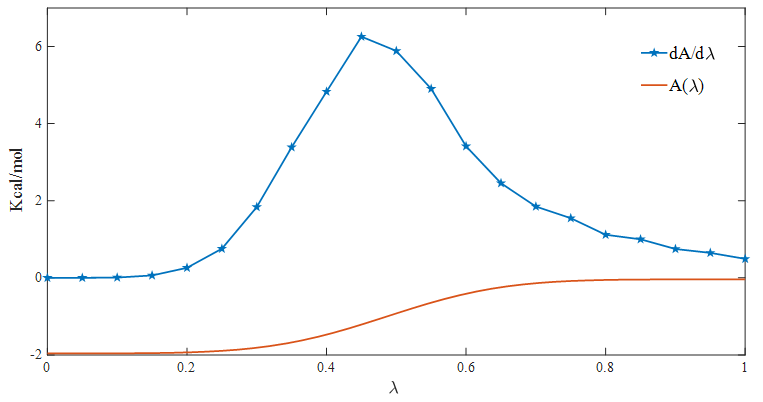
\includegraphics[width=0.95\linewidth]{RFEP}
    \caption{Restraint free energy ($\Delta G_\lambda)$, top) and its derivative with respect to the coupling parameter ($\partial G/\partial\lambda$, bottom), as a function of $\lambda$. Error bars indicate standard deviation of the mean.
    }\label{fig:RFEP2}
\end{figure}
As in FEP, restraint free energy perturbation (RFEP) scales certain energy terms and the associated forces using a perturbation parameter, $\lambda\in \{0,1\}$.
The main difference between FEP and thermodynamic integration (TI), is that FEP estimates finite free energy differences between $\lambda$ values while TI calculates the derivatives. This is possible because the force constant, $k$, depends directly on lambda:
 \begin{equation}\label{eq:kl}
     k_\lambda = k_0 + \lambda^\alpha (k_1-k_0)
 \end{equation}
Where $k_0 = 0$ is the force constant (\texttt{forceConstant}) when $\lambda=0$, $k_1$ is the  force constant when $\lambda=1$ (\texttt{targetForceConstant}), and $\alpha$ (\texttt{targetForceExponent}) is a tuning parameter that improves convergence of TI by making the energy a smoother function of $\lambda$ near $\lambda=0$.

Combining Equations~\ref{eq:harmonicWall} and \ref{eq:kl} and taking the partial derivative with respect to $\lambda$ yields:
\begin{equation}\label{eq:dUwalldlambda}
    \frac{\partial}{\partial \lambda} U_\mathrm{FW}(\lambda, \xi) =\begin{cases}
        \frac{1}{2}\alpha\lambda^{\alpha-1}(k_1 - k_0)(\xi-\xi_\mathrm{max})^2&, \xi>\xi_\mathrm{max}\\
        0 &, \text{otherwise}
    \end{cases} 
\end{equation}
Where $k$ in Equation \ref{eq:harmonicWall} is replaced by $k_\lambda$ in Equation~\ref{eq:kl}.
In \ref{step:restraintPerturbation}, $\xi$ is replaced by $d$, the DBC, and $\xi_\mathrm{max}$ is replaced by the upper wall of the DBC restraint, $d_\mathrm{max}$.
%where $\xi$ in Equation \ref{eq:harmonicWall} is replaced by the DBC, and $d_\mathrm{max}$ is the upper wall of the DBC restraint.
This is applied to the colvars trajectory data in the Jupyter notebook section associated with Step C. 

By integrating over the expectation value of the gradient, as derived and discussed in most statistical mechanics and molecular dynamics textbooks (e.g. \cite{Tuckerman2010, frenkel2001understanding}), we obtain the Helmholtz free energy:
\begin{align}\label{eq:thermodynamicintegration}
    \Delta F &= \int_{0}^{1} \left< \frac{\partial U_\mathrm{FW}}{\partial \lambda} \right>_{\lambda} d\lambda\\
    &\approx \Delta G , P\Delta V \approx 0
\end{align}
Which can be approximated numerically by discretizing and summing over $\lambda\in\{0,1\}$:
\begin{equation} \label{eq:TI}
    \Delta G = \sum_{\lambda=0}^1 \left\langle
    \frac{\partial U(\lambda)}{\partial \lambda}\right\rangle
\end{equation}

Finally, the error is estimated using the standard deviation of each mean (as seen in Figure \ref{fig:RFEP2}). A more accurate estimate of the error can be obtained by running replicas of the TI calculation. 
Further details can be found in the provided configuration files and in \ref{step:restraintPerturbation} of the protocol.


\section{Concentration Dependence and Non-Ideality} \label{app:bindingProbability}

While in this tutorial we have only used a single, infinitely dilute, concentration to calculate  $\Delta G_\mathrm{bind}$, SAFEP can also be used to predict concentration dependence in non-ideal and non-dilute solutions.  Here we consider the underlying theory for interpreting such a calculation, and provide general suggestions for implementation.

We consider a ``unitary'' (single protein, single site\cite{Salari2018}) system with $m$ ligands in a volume $V$. The ligand concentration in this system is $L=m/V$. A DBC coordinate $d_i$ can be defined for each of the $m$ ligands, indexed by $i$.  

The threshold on the DBC coordinate meaningfully divides the ensemble into two possible macrostates: occupied (one ligand occupies the site and $m-1$ ligands are in solution) and unoccupied (no ligands occupy the site and $m$ ligands are in solution.)  We formalize this here through the DBC ``test function,'' which for an individual ligand $i$ is a Heaviside step function  of the form 
\begin{align} 
   \Theta_i &= \begin{cases}
        1 &, \; d_{i} < d_\mathrm{max}\\
        0 &, \; \text{otherwise}
    \end{cases}
\end{align}
The instantaneous site occupancy $\Theta_\mathrm{occ}$ is determined by whether any of the $m$ ligands occupy the site, given by the sum of all the individual test functions:
\begin{equation}
   \Theta_\mathrm{occ}=\sum_{i=1}^m\Theta_i. 
\end{equation}
Since here we consider the case where the site can bind at most one ligand, $\Theta_\mathrm{occ}$ is either 0 or 1.  

The  partition functions for the occupied and unoccupied states are thus $Z_\mathrm{occ}$ and $Z_{unocc}$ respectively, where 
\begin{align}
    Z_{\mathrm{occ}} &=\int \Theta_\mathrm{occ}e^{-\beta U} \mathrm{d}^N\vec{r}\\ 
    Z_{\mathrm{unocc}} &= \int \left[1-\Theta_\mathrm{occ}\right]e^{-\beta U} \mathrm{d}^N\vec{r} , 
\end{align}
and the potential energy $U$ is a function of the positions $\vec{r}$ of all $N$ particles in the system, while $\Theta_\mathrm{occ}$ is a function of the DBC coordinates $d$ (and thus the positions of ligand and site atoms only).  

The occupancy probability $P_\mathrm{occ}(L)$ is thus  
\begin{align}\label{eq:probability1.5}
    P_\mathrm{occ}(L)=\frac{Z_{\mathrm{occ}}} {Z_{\mathrm{occ}} + Z_{\mathrm{unocc}}}=\frac{\int \Theta_\mathrm{occ} e^{-\beta U} \mathrm{d}^N\vec{r}} {\int e^{-\beta U}\mathrm{d}^N\vec{r}}=\langle \Theta_\mathrm{occ}\rangle
\end{align} 
which, as expected, yields the average occupancy $\langle \Theta_\mathrm{occ}\rangle$.  

Each macrostate has an associated free energy: 
\begin{align}
    \beta G_\mathrm{occ}&=-\ln Z_\mathrm{occ}\\
    \beta G_\mathrm{unocc}&=-\ln Z_\mathrm{unocc},
\end{align}
where $G_\mathrm{occ}$ and $G_\mathrm{unocc}$ are the free energies of the occupied and unoccupied macrostate respectively, so 
\begin{align}
    P_\mathrm{occ}(L)=\frac{e^{-\beta G_\mathrm{occ}}} {e^{-\beta G_\mathrm{occ}} + e^{-\beta G_\mathrm{unocc}}}.\label{eq:ApE:probability2}
\end{align}

We turn now to connecting these quantities to a SAFEP calculation.  In step D of the protocol, we decoupled one ligand from a bulk that contained $m=0$ fully coupled ligands, for an infinitely dilute concentration of $L=0/V$. We then extrapolated to the standard concentration using an ideal gas correction that assumes ideality.

For a ligand at finite concentration in a non-ideal bulk, it is not useful or necessary to standardize the free energy. Instead, we would carry out Step D at the finite ligand concentrations of interest ($L=m/V>0$), and adjust Step E to calculate the unstandardized free energy $\Delta G_\mathrm{bind}(L)$ as follows: 
\begin{equation}
\Delta G_\mathrm{bind}(L)= - \Delta G_\mathrm{site}^* + \Delta G_\mathrm{DBC} -\Delta G_\mathrm{V}(L)+ \Delta G^*_\mathrm{bulk}(L)
\end{equation} 
where the volume per molecule in the bulk is $V/m$ and thus \begin{equation}
\label{eq:idealGas}
    \Delta G_\mathrm{V}= -\frac{1}{\beta} \ln \frac{m V_\mathrm{R}}{V}. 
\end{equation}
Since
    $\Delta G_\mathrm{bind}(L) = G_\mathrm{occ}(L) - G_\mathrm{unocc}(L)$

Equation \ref{eq:ApE:probability2} can be rewritten in terms of $\Delta G_\mathrm{bind}(L)$:  
\begin{align}
 P_\mathrm{occ}(L) = \frac{1}{1+e^{\beta \Delta G_\mathrm{bind}(L)}} \label{eq:ApE:probability3}
\end{align}
Even for a non-ideal bulk, we may assume the excess chemical potential is unchanging for small changes in concentration. Thus we may perform ligand decoupling (step D) at finite concentration $L$, and use the ideal gas correction to predict occupancy for nearby concentrations $L^\prime$, as long as $|L-L^\prime|$ is small.
\begin{equation}
\label{eq:concentrationShift}
    \Delta G_\mathrm{bind}(L^\prime)= \Delta G_\mathrm{bind}(L)-\frac{1}{\beta} \ln \frac{L^\prime}{L}
\end{equation}
Substitution of Equation \ref{eq:concentrationShift} in Equation \ref{eq:ApE:probability3} yields the occupancy probability for concentration $L^\prime$:
\begin{equation}\label{eq:bindingStatmech}
    P_\mathrm{occ}(L^\prime)\sim\frac{L^\prime}{L^\prime+{L}e^{\beta \Delta G_\mathrm{bind}(L)}}
    \end{equation} 
Incidentally, for dilute $L$, ${L}e^{\beta \Delta G_\mathrm{bind}(L)}={L^\circ}e^{\beta \Delta G^\circ_\mathrm{bind}}=K_d$,
and Equation~\ref{eq:bindingStatmech} reduces to  a form familiar to biochemists 
$
    P_\mathrm{occ}(L^\prime)~=~\rm\frac{L^\prime}{L^\prime+K_d}.
$
In general, Equation \ref{eq:concentrationShift} only holds if the change in excess chemical potential is negligible between $L^\prime$ and the simulation concentration $L$.
This assumption can be tested by running bulk decoupling (Step D) at both $L^\prime$ and $L$ and checking that the resulting change in $\Delta G_\mathrm{bulk}$ is much smaller than the overall error. If we wish to calculate $P_\mathrm{occ}$ over a wider concentration range where this assumption does not hold, we would need to explicitly calculate $\Delta G^*_\mathrm{bulk}(L)$ for multiple simulation concentrations $L$ and extrapolate to the intermediate concentrations, as in Ref. \cite{Salari2018}.

\onecolumn
\section{Checklist}
\label{app:checklist}
\begin{Checklists*}

\begin{checklist}{Infrastructure}
\textbf{Because of the complexity and investment required for FEP calculations, it is important to keep files well-organized and to optimize run conditions to avoid wasted compute time.}
\begin{itemize}
\item (first time) Find the location of a FEP- and Colvars-compatible NAMD installation.
\item Determine the optimal run settings by benchmarking the bound complex and the solvated ligand.
\item Organize the inputs, run scripts, and config files (The GitHub of this tutorial is just one possible organization scheme, but your needs may vary.)
\end{itemize}
\end{checklist}

\begin{checklist}{System Selection and Modeling}
\textbf{The quality of the free energy estimate will depend on the quality of the initial conditions.}
\begin{itemize}
\item Model or obtain a model of the protein-ligand complex
\item Model or obtain a model of the free ligand
\item Parameterize and solvate the systems (e.g. using CHARMM-GUI or similar)
\item Relax the models. The outputs will be the starting points for later simulations.
\end{itemize}
\end{checklist}

\begin{checklist}{Determine the DBC}
\textbf{Parameterization of the DBC depends on a well-sampled unbiased simulation and some trial and error in choosing the restrained atoms. Additional unbiased simulations may be necessary to understand the unbound ensembles of the protein and ligand. It is critical that the \textit{definition }of the DBC is identical in \textit{all} simulations.}
\begin{itemize}
\item Run a ``long'' simulation of the bound ensemble (at least 50~ns)
\item Check standard measures of equilibration (e.g. RMSD or box size)
\item Choose a stable subset of the heavy atoms of the ligand to constitute the DBC.
\item Examine the DBC trajectory and histogram using this definition.
\item Vary the atoms in the DBC until the distribution becomes sufficiently narrow (5 or 6 $\AA$ is a rough upper limit of feasibility).
\end{itemize}
\end{checklist}

\begin{checklist}{Run FEP in the Site}
\begin{itemize}
\item Specify the atoms to be decoupled
\item Choose a lambda schedule and length for each window
\item Run the FEP
\item Examine the trajectory for any abnormal behaviors
\item Check the trajectory of the DBC and DBC restraint
\item Analyze the fepout file to obtain $\Delta G^*_\mathrm{site}$
\end{itemize}
\end{checklist}

\begin{checklist}{Run TI}
\begin{itemize}
\item Confirm that the DBC used here is the exact same as was used in FEP
\item Design the isotropic (COM) restraint
\item Choose a lambda schedule and length for each window of the DBC TI
\item Run the TI
\item Examine the trajectory for any abnormal behaviors
\item Check the trajectory of the collective variables and restraints
\item Analyze the colvars.traj file to obtain $\Delta G_\mathrm{DBC}$
\end{itemize}
\end{checklist}
\end{Checklists*}

\begin{Checklists*}
\begin{checklist}{}\end{checklist}
\begin{checklist}{Run FEP in the Bulk}
\begin{itemize}
\item Specify the atoms to be decoupled
\item Choose a lambda schedule and length for each window of the DBC TI
\item Run the FEP
\item Examine the trajectory for any abnormal behaviors
\item Check the trajectory of the collective variables and restraints
\item Analyze the colvars.traj file to obtain $\Delta G^*_\mathrm{bulk}$
\end{itemize}
\end{checklist}

\begin{checklist}{Calculate Analytical Corrections and Combine}
\begin{itemize}
\item Calculate the ideal gas contribution ($\Delta G_V$)
\item Calculate any other analytical corrections (e.g. charge)
\item Combine values and errors to get the $\Delta G^\circ_\mathrm{bind}$
\item Plot the titration curve
\item Compare the result with known quantities
\end{itemize}
\end{checklist}

\end{Checklists*}

\twocolumn
\section{Troubleshooting}
\label{app:troubleshooting}
We have written this tutorial to be as robust as possible but also generalizable to other systems. 
In the process of applying these steps to your own system of interest, however, additional challenges may arise. 
When calculations fail to converge or appear to converge to unreasonable values, it can be difficult to discern what has gone wrong without simply starting over. 
We provide here some of the most common issues and their respective fingerprints as cautionary tales and troubleshooting tools. 
If you encounter a problem with running the tutorial as written and do not see your issue listed below, please contact us.

\subsection{Problems with Running; NAMD crashes}
Alchemical FEP will make any instabilities in a system more apparent as well as introduce a few more possible sources of instability. The most common problems are RATTLE errors and box size instability

\subsubsection{RATTLE Errors}
\begin{quote}
\texttt{ERROR: Constraint failure in RATTLE algorithm for atom 593!}
\end{quote}

\noindent\textbf{Causes:}

If the usual culprits (poor equilibration, long time steps, and over-aggressive RESPA settings) have been ruled out, the most likely causes of RATTLE errors during FEP are 1) too-wide lambda windows and 2) a too-low soft-core potential exponent.

\noindent\textbf{Solutions:}

Lambda windows can easily be narrowed by reducing \textInput{dLambda}. Values between 0.05 and 0.005 give a good balance between efficiency and accuracy.
Note, the shorter the windows, the more windows that will be run and the more CPU time required to complete the calculation.

The soft-core potential (\textInput{alchVdwShiftCoeff}) should be between 5 and 10. Although higher values are ``softer'' and so avoid end-point ``catastrophes,'' they are also prone to under-estimate energy differences.

\subsubsection{Box Size Instability}
\begin{quote}
\texttt{FATAL ERROR: Periodic cell has become too small for original patch grid!}

\texttt{Possible solutions are to restart from a recent checkpoint,
increase margin, or disable useFlexibleCell for liquid simulation.}
\end{quote}

\noindent\textbf{Causes:}

While classical MD is ``tolerant'' to small periodic boxes and aggressive barostats, combining these with FEP is particularly unstable.

\noindent\textbf{Solutions:}

First, the periodic box should be at least twice the solute size or twice the cutoff distance (whichever is longer) this will avoid self-interactions which can cause instabilities especially with charged solutes and during FEP decoupling. Second, at least with the Langevin barostat, slowing the piston dynamics can improve system stability but slows box relaxation. We use \textInput{LangevinPistonPeriod} between 75 and 200, and \textInput{LangevinPistonDecay} between 50 and 100. \textInput{LangevinPistonDecay} should always be about half \textInput{LangevinPistonPeriod}. See \href{https://www.ks.uiuc.edu/Research/namd/2.14/ug/node39.html}{The NAMD UG} for more details. \cite{Bernardi2020}





\subsection{Problems with Results; Poor Convergence}

Convergence within each step is a prerequisite to a good final estimate of $\Delta G^\circ_\mathrm{bind}$. Large errors and internal inconsistencies often indicate poor equilibration or under-sampling of one or more ensembles. Each leg of a SAFEP calculation has unique challenges and edge-cases which we address below. 

In general, convergence may be improved by increasing the simulation time for each lambda value.

\subsubsection{Local and Misleading Convergence}
In the case of very slow fluctuations or in the presence of metastable states, a FEP calculation may be converge locally and give a biased outcome.
The best way to detect this is to run multiple replicas as uncorrelated from one another as possible. 
% There are two main ways to assess bias in a given sample. 
% The first is to simply run multiple replicas as uncorrelated from one another as possible. 
% The second is to run unbiased simulations of each of the intermediate states and compare those ensembles to the ensembles obtained during FEP or TI calculation. \jh{I don't get this}
% \jh{the use of biased / unbiased above is unclear}

In this tutorial, we include analysis of the protein-ligand bound state ensemble because it directly affects the definition of the DBC.
Simulation of the apo protein (without ligand in the binding pocket), however, can provide useful information about the decoupled end-point.
In the case of lysozyme, for example, the binding pocket is frequently occupied by one or two water molecules.
If the lysozyme binding pocket does not recover hydration once the ligand is fully decoupled during FEP, the calculation overestimates the strength of binding by up to 0.5~kcal/mol. This is a small error compared to the overall precision of the technique, but users should be aware that assessing endpoint hydration is particularly important for larger or more hydrated binding pockets. 

\subsubsection{Step A: Define the DBC}
\noindent\textbf{Symptom:}  Multimodal DBC Distribution (e.g. Figure \ref{fig:bimodalDBC})\\
\begin{figure}[!htb]
    \centering
    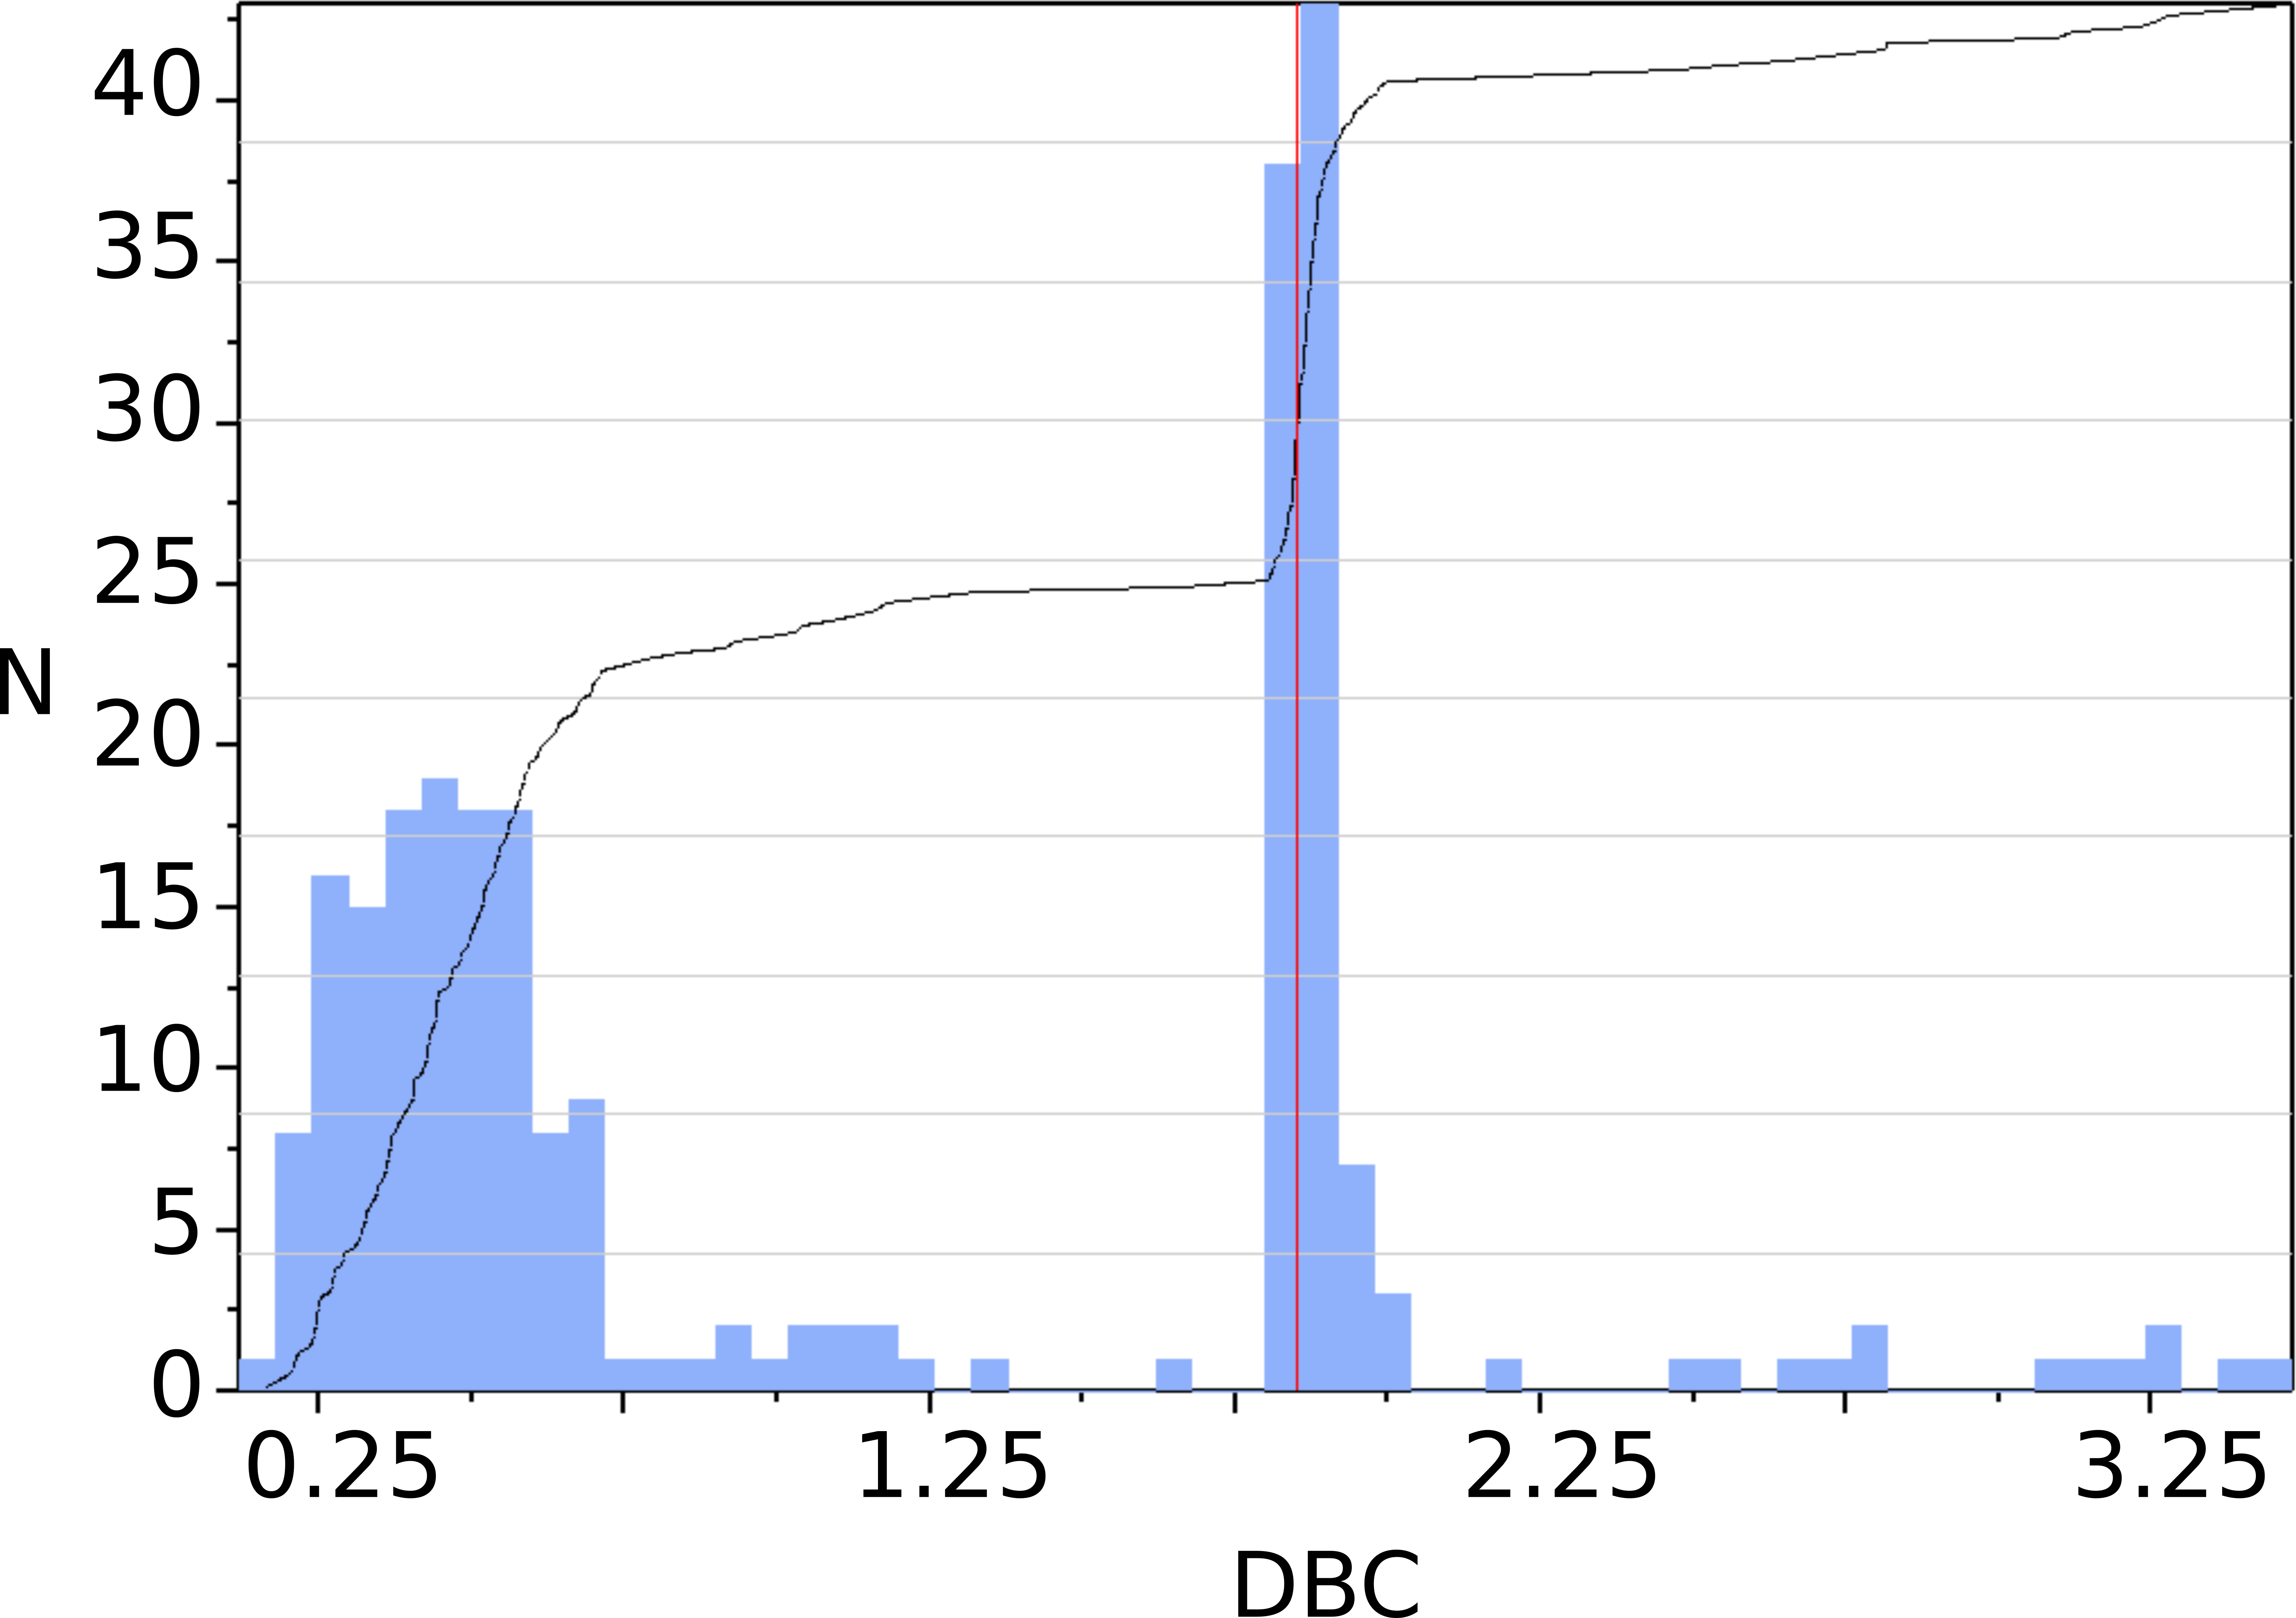
\includegraphics[width=0.9\linewidth]{Figures/recropped_bimodal.png}
    \caption{Screenshot from the Colvars Dashboard showing a bimodal distribution that resulted from using an asymmetric DBC for phenol. The second peak corresponds to a 180~degree rotation about the C-O axis.}
    \label{fig:bimodalDBC}
\end{figure}
\noindent\textbf{Causes:}\\
There are three main causes of multimodal DBC distributions: 1) ligand unbinding, 2) multiple binding modes, and 3) multiple, nearby binding sites.\\ 
\textbf{Solutions:}\\
Use the Colvars Dashboard histogram tool to probe the conformations associated with each mode and decide which modes correspond to bound and unbound states. \\
\begin{tabular}{|p{3cm}|p{5cm}|}
    \hline
    \center Bound and Unbound modes & If all but one mode may be described as unbound, place the DBC restraint between the bound mode and the least unbound mode. Proceed with FEP. \\\hline
    \center Multiple, indistinguishable bound modes & Such modes are a result of symmetric ligands and are best addressed using a symmetric DBC. See \ref{app:Symmetry} for more details.\\\hline
    \center Multiple, distinguishable bound modes & If one or more bound mode(s) is meaningfully distinct from some other mode(s), select a representative frame for each class. These frames become reference poses for each binding ``site'' from which you must calculate $\Delta G_\mathrm{site}$, $\Delta G_\mathrm{DBC}$, and $\Delta G_\mathrm{V}$ separately. Free energy contributions from each mode can be combined by exponential averaging as shown in equation 12 of \cite{Mobley2006}. \\\hline
\end{tabular}


\subsubsection{Step B or D: FEP Calculations}
\noindent\textbf{Symptom:}  DBC energy starts low and stays low\\
\textbf{Causes:}\\
the DBC may be too wide/soft. The lambda windows may be too short to properly sample the decoupled ensemble.\\
\textbf{Solutions:}\\
First, watch the trajectory for any abnormal behavior; wide DBCs will often be obvious from the last several nanoseconds of a FEP run because the ligand will move quickly around the box. Then see the DBC debugging list below. If the system passes all checks, try running $\lambda=1$ for longer to make sure the DBC restraint is functioning.\\

\noindent\textbf{Symptom:} DBC energy is consistently greater than 0\\
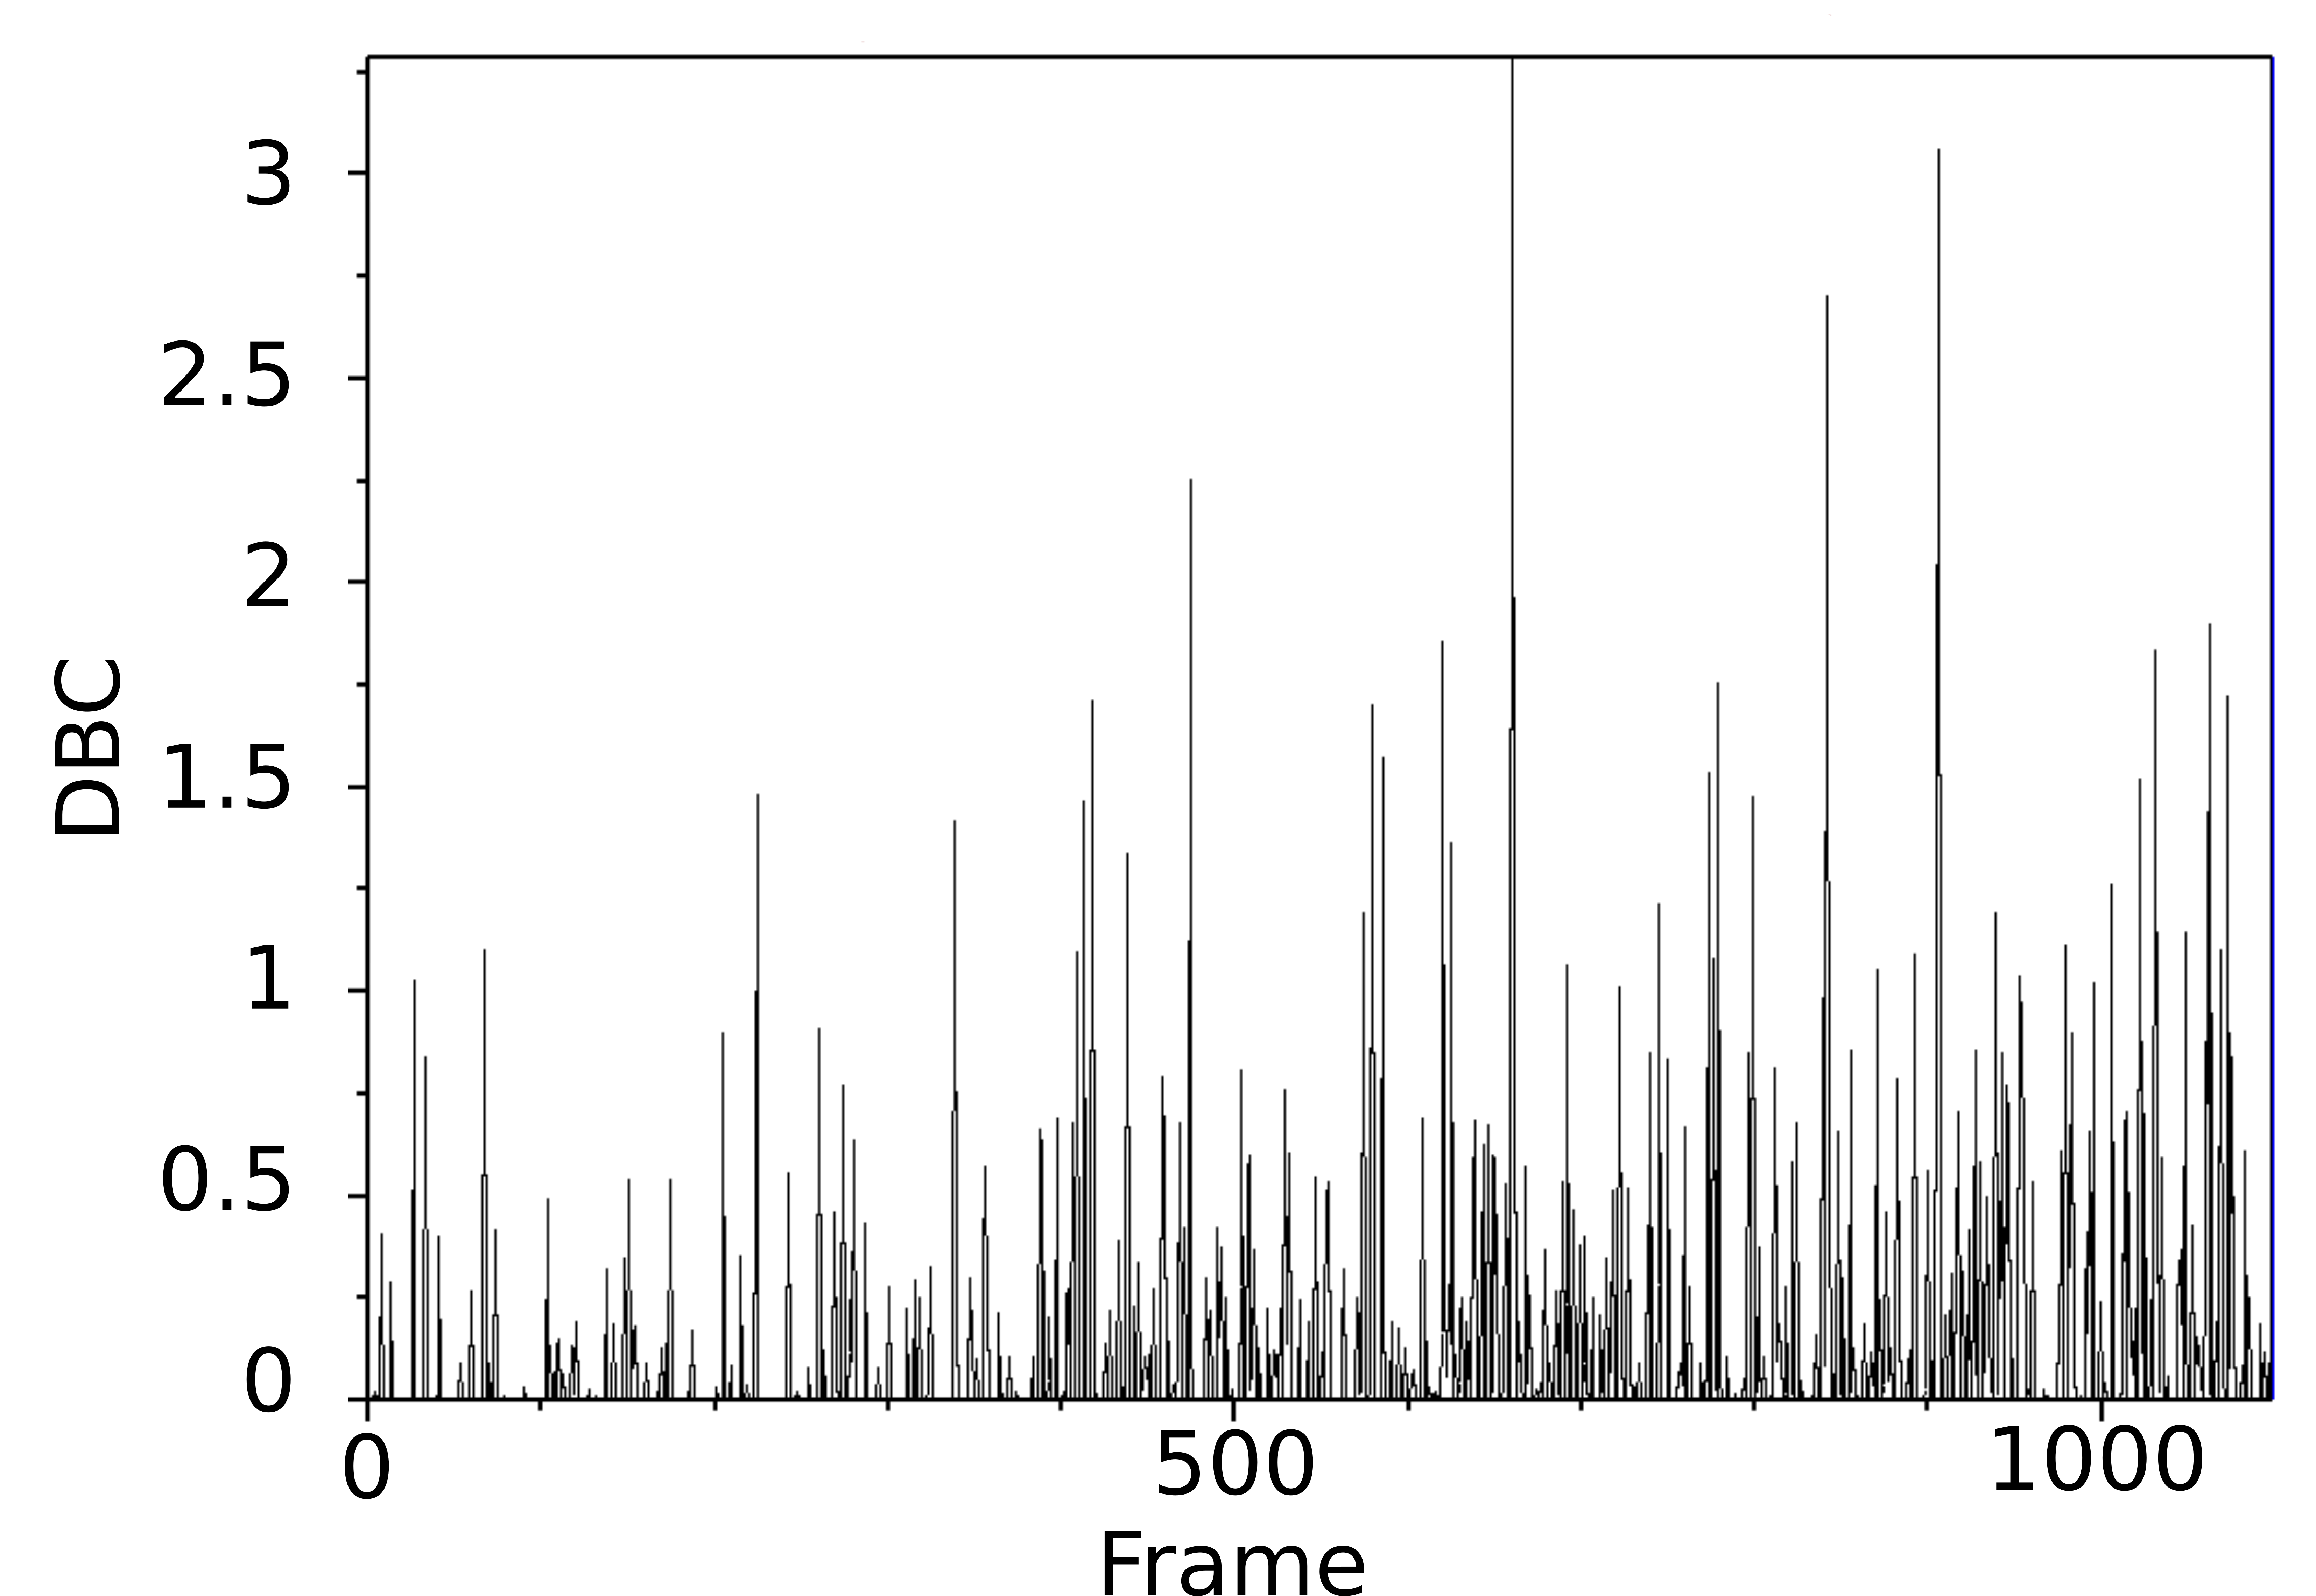
\includegraphics[width=0.9\linewidth]{tightDBC_alchsite.png}
\textbf{Causes:}\\
This issue is most often due to too-narrow DBC restraints or mistakes in the Colvar definition.\\
\textbf{Solutions:}\\
This problem is harder to diagnose from the trajectory alone unless there are obviously over-restrained degrees of freedom in the ligand. Consult the DBC debugging checklist below.

\noindent\textbf{Symptom:} Ligand Unbinding during FEP\\
\textbf{Cause:}\\
The most likely cause of unbinding during FEP is a DBC restraint that is too broad or too weak.\\
\textbf{Solutions:}\\
 Consult the DBC debugging checklist:\\

\textbf{DBC Debugging Checklist:}
\begin{todolist} \label{list:DBCdebug}
    \item Only the DBC restraint should be active during FEP (\ref{step:proteinDecouple})
    \item DBC restraint upper walls have the right value. (\ref{step:createDBC})
    \item DBC restraint force constant is appropriate (100 or 200). (\ref{step:createDBC})
    \item NO lower walls (\ref{step:createDBC})
    \item If the Colvars configuration file contains a ``width'' keyword, it should be 1. See \cite{Fiorin2013} and the \href{http://colvars.github.io/colvars-refman-vmd/colvars-refman-vmd.html#sec:colvar_grid_params}{Colvars user guide} for more details. (\ref{step:createDBC})
\end{todolist}


\noindent\textbf{Symptom:} Very Large Hysteresis near $\lambda=0.5$\\
Hysteresis ($\delta_\lambda$) larger than 1~kcal/mol for any lambda window suggests poor convergence.\\
\textbf{Causes:}\\
Large hysteresis values are most often caused by: 1) insufficient equilibration, 2) short windows (less than a few hundred ps), or 3) wide windows (large $d\lambda$).\\
\textbf{Solutions:}\\
If the system is well-relaxed and equilibrated by the usual metrics (box size, pressure, temperature, etc.), then it is most likely that either the lambda windows are too short or too wide. Try increasing the sampling time or increasing the total number of windows. We have had good results with 120 windows of 3~ns each but longer may be necessary for particularly unwieldy systems.\\

\noindent\textbf{Symptom:}  Very Large Hysteresis near $\lambda=0$ or $\lambda=1$\\
\textbf{Causes:}\\
Large hysteresis near the end-points of the FEP calculation are most commonly caused by so-called ``end-point catastrophes.'' See \href{https://www.ks.uiuc.edu/Research/namd/2.14/ug/node63.html}{The NAMD UG} for more details. \cite{Bernardi2020}\\  
\textbf{Solutions:}\\
The first parameter to check is \textInput{alchVdwShiftCoeff}. As noted above, it should be between 5 and 8. If this is already the case, and no other part of the calculation is problematic, try doubling the number of windows between the window with large hysteresis and the nearest end-point.\\

\noindent\textbf{Symptom:}  Hysteresis Oscillates or is Otherwise Correlated with $\lambda$.\\
As noted above, $\delta_\lambda$ should be independent of lambda with a mean of 0.\\
\textbf{Causes:}\\
Some versions of NAMD have a bug that allows FEP data to be written on a step without energy calculations. This results in the use of stale energies (from a previous step) and inaccurate estimates for differences in energy.\\
\textbf{Solutions:}\\
Manually ensure that \textInput{alchOutFreq} is a multiple of both \textInput{fullElectFrequency} and \textInput{nonbondedFreq}. See \href{https://www.ks.uiuc.edu/Research/namd/mailing_list/namd-l.2020-2021/1487.html}{Bug advisory and Workaround} for more details.\\


\subsubsection{Step C: TI Calculation}
The DBC restraint should do the most work early in the TI calculation then, as the force constant is scaled out, the COM restraint should take over and keep the center of mass in a well-defined volume. TI convergence issues are most easily diagnosed by watching the MD trajectory and examining the colvar trajectories.

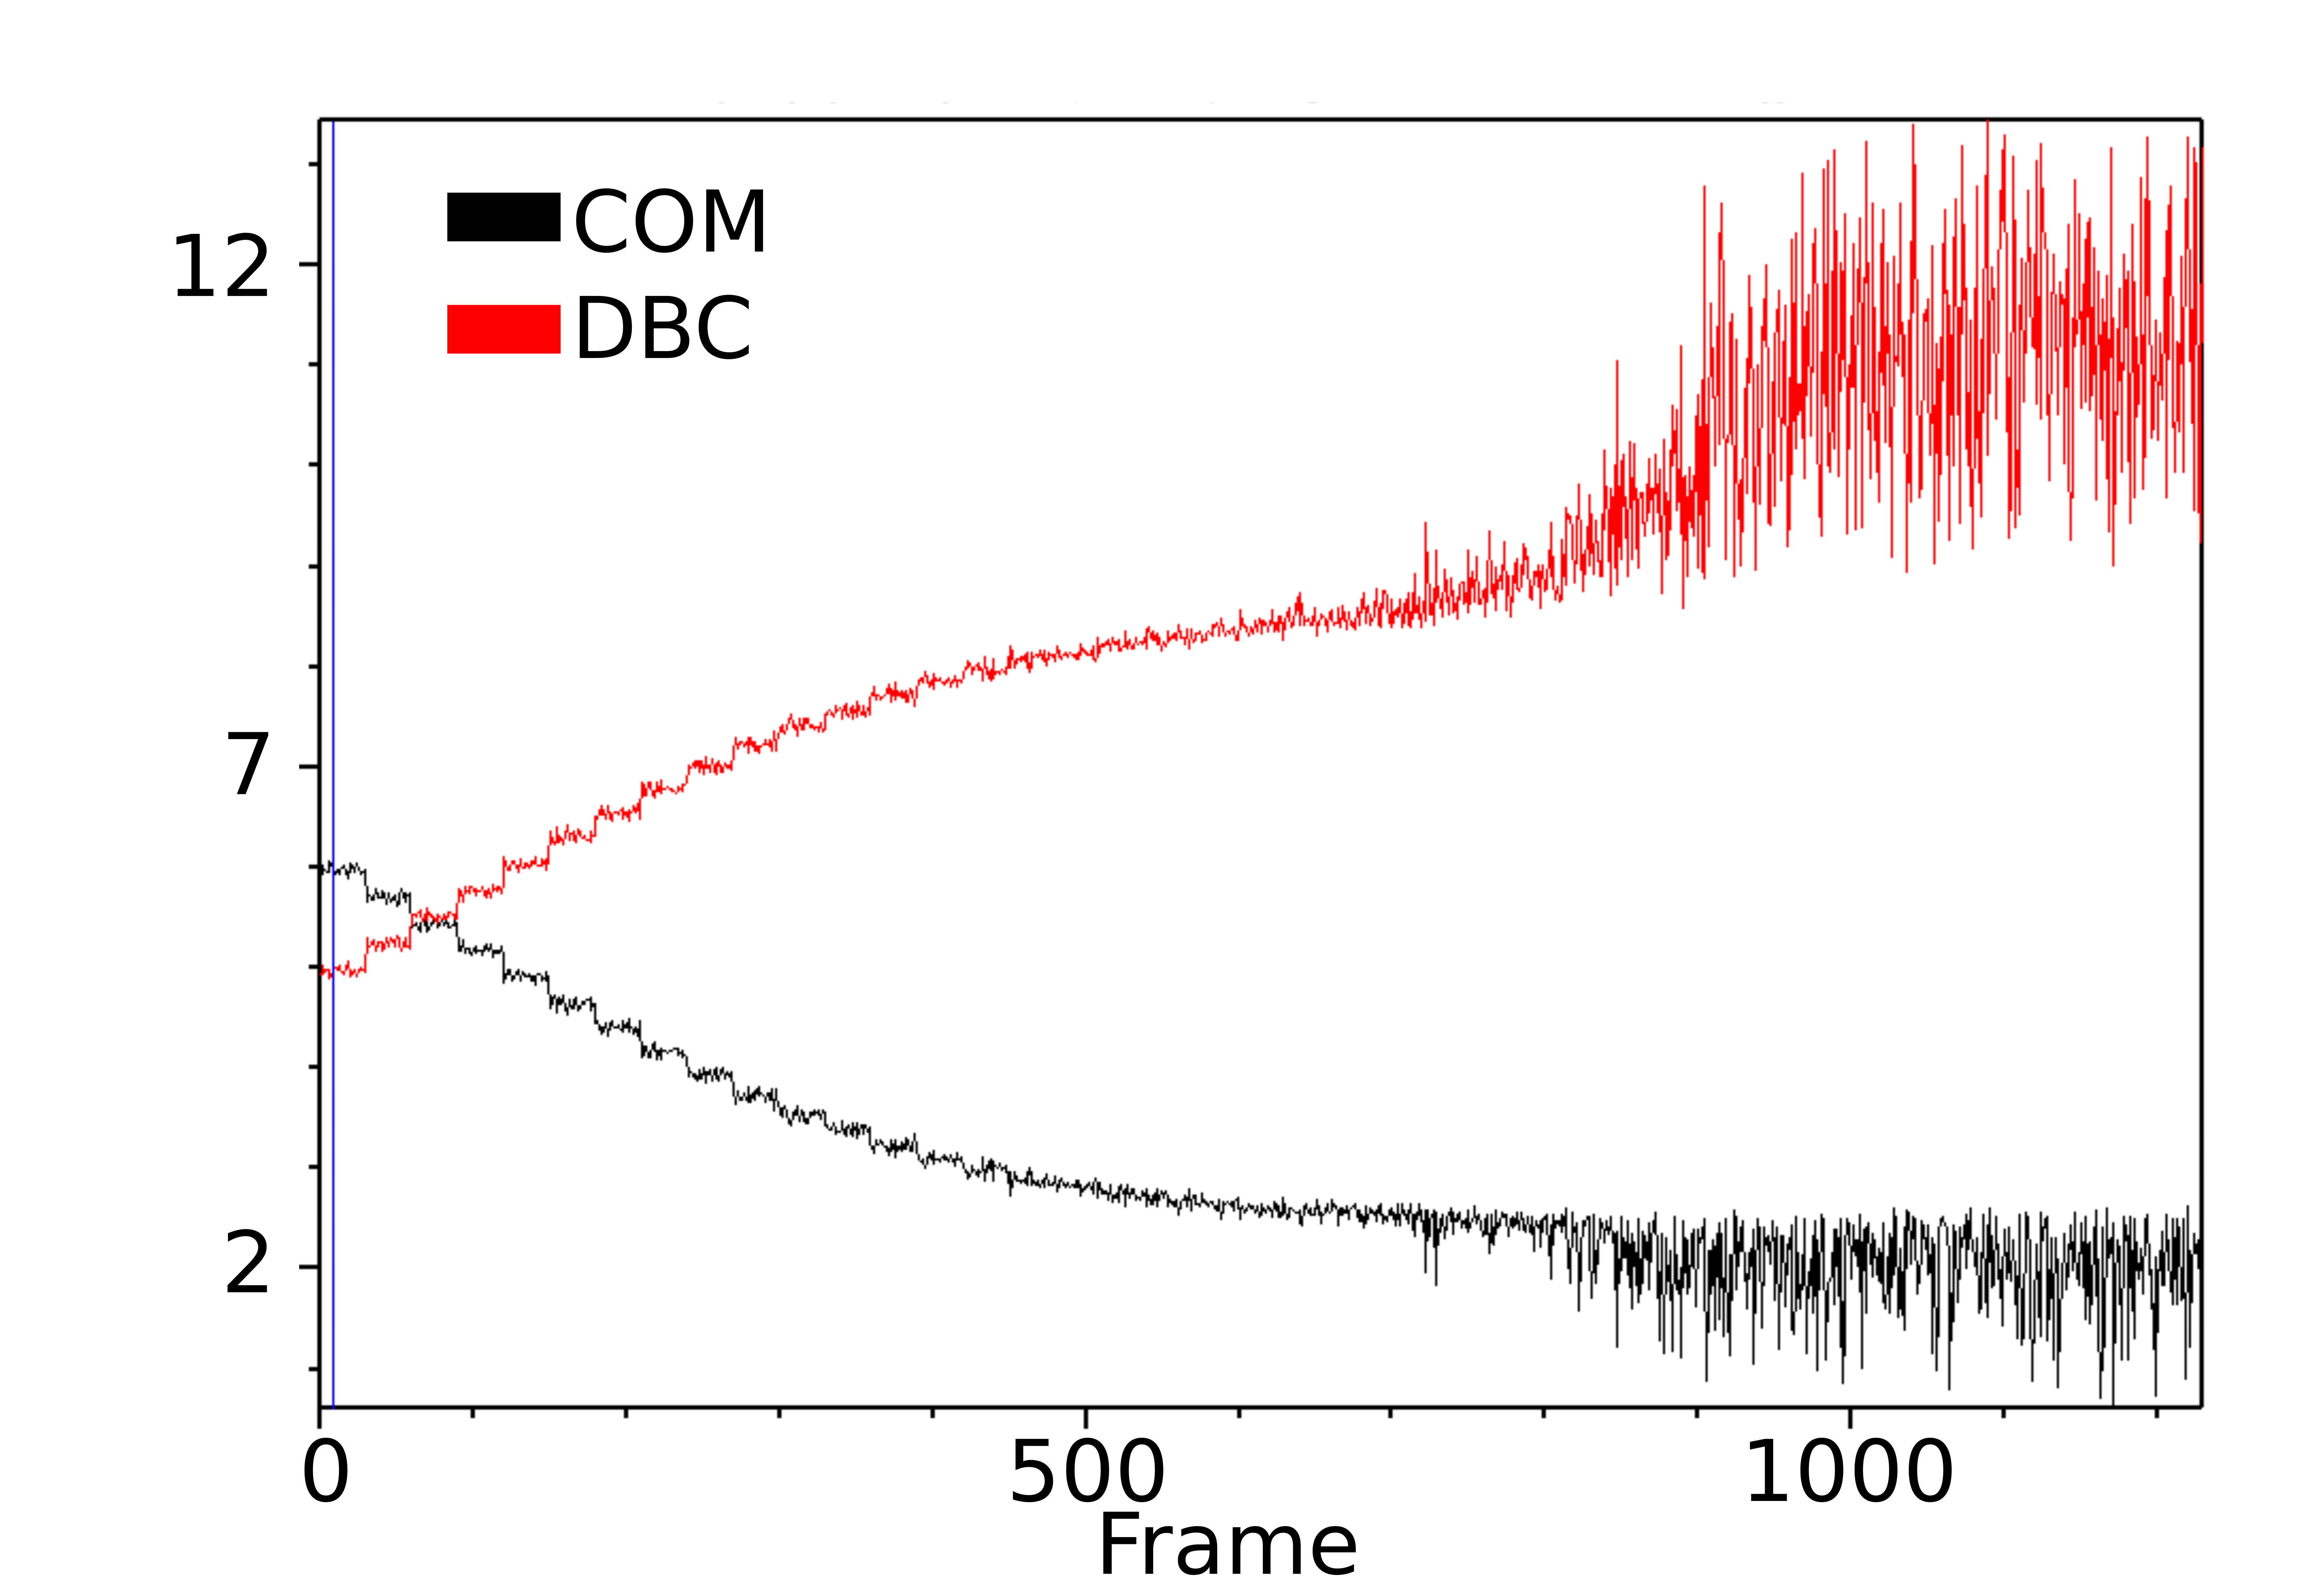
\includegraphics[width=0.9\linewidth]{CV_COM_mismatchedRefs.png}

\noindent\textbf{Symptom:} The collective variable trajectory is abnormal\\
\textbf{Causes:}\\
Strange behavior is expected if you over-write the sample outputs and attempt to run with \textInput{useSampleFiles} set to 1. The example above is the result of a mismatch between the coordinates used to determine the center of the COM restraint and the reference coordinates used for the DBC restraint.\\
\textbf{Solutions:}\\
Update the reference coordinates to match those used for determining the center of the COM restraint. That is, revisit Step C\hyperref[step:defineGasRestraints]{1.b} paying special attention to the coordinates used. Make sure you save your files in the correct directories. \\

\noindent\textbf{Symptom:} Restraint energies during TI are very high or very low and don't change much\\
\textbf{Causes:}\\
The harmonic walls are likely too stiff or too soft.\\
\textbf{Solutions:}\\
Adjust the force constants to be between 100 (minimum) and 200. \\

\noindent\textbf{Symptom:} The ligand doesn't move during TI (or moves very little)\\
\textbf{Causes:}\\
The restraints are probably too narrow.\\
\textbf{Solutions:}\\
Double check the choice of wall position and ensure that it is correct in all Colvar config files.\\

\noindent\textbf{Symptom:} The ligand flies away during TI (and the calculation doesn't converge)\\
\textbf{Causes:}\\
The restraints are probably too wide.\\
\textbf{Solutions:}\\
Double check the choice of wall position and ensure that it is correct in all Colvars config files.\\



\setcounter{section}{3}
\renewcommand\thesection{\arabic{section}}
\section{Author Contributions}
ESM, ME and JWS ran, tested and refined the protocol.
ESM wrote the notebook and analysis scripts.
GB and JH designed and supervised the work.
All authors wrote the document.

\section{Other Contributions}
The authors are grateful to 
Ms. Noureen Abdelrahman, 
Ms. Mariadelia Arg\"uello-Acu\~na,
Mr. Jahmal Ennis, 
and
Mr. Connor Pitman for providing feedback and initial testing of this tutorial. The authors acknowledge the Office of Advanced Research Computing (OARC) at Rutgers, The State University of New Jersey for providing access to the Amarel cluster and associated research computing resources. 

\section{Potentially Conflicting Interests}
The authors declare no potential conflict of interests.


\section{Funding Information}
We acknowledge financial support from the National Science Foundation DGE 2152059 (to ESM, JWS, and GB), the Ministry of Science, Research, and Technology of the Islamic Republic of Iran for a Ph.D. candidate research grant to ME, and the French Agence Nationale de la Recherche (ANR) for grant LABEX DYNAMO (ANR-11-LABX-0011-01, to JH).

\section*{Author Information}
\makeorcid

% \bibliographystyle{plain}
\bibliography{Ref}
\end{document}
